%% Elsevier elsarticle template (authoryear / Harvard)
%% English version of Paper 1 (generalization focus, NO adversarial).
%% Source (Indonesian): paper1-generalisasi.tex (adversarialfalse).
%% All numbers come from real, reproducible experiments.

\documentclass[preprint,12pt,authoryear]{elsarticle}

\usepackage{amssymb}
\usepackage{amsmath}
\usepackage{booktabs}
\usepackage{multirow}
\usepackage{siunitx}
\usepackage{graphicx}
\usepackage{algorithm}
\usepackage{algpseudocode}
\usepackage{tikz}
\usetikzlibrary{arrows.meta,positioning,fit,backgrounds}
\graphicspath{{figure-q1/}}

\journal{Journal of Information Security and Applications}

\begin{document}

\begin{frontmatter}

\title{Semantic Feature Mapping and Few-Shot Calibration for Cross-Network
Intrusion Detection}

\author[pens]{Hero Yudo Martono\corref{cor1}}
\ead{hero@pens.ac.id}
\author[pens]{Iwan Syarif}
\ead{iwanarif@pens.ac.id}
\author[pens]{Ferry Astika Saputra}
\ead{ferryas@pens.ac.id}
\cortext[cor1]{Corresponding author.}

\affiliation[pens]{organization={Department of Informatics and Computer, Politeknik Elektronika Negeri Surabaya (PENS)},
            city={Surabaya},
            country={Indonesia}}

% Highlights are submitted as a SEPARATE item per Elsevier/JISA rules
% (3-5 bullets, each <= 85 chars). Source file: highlights.tex (in this repo).
%
% Graphical Abstract is submitted as a SEPARATE image file per JISA/Elsevier rules
% (EPS/PDF/TIFF, ~531x1328 px), NOT embedded in the manuscript. Source figure:
% graphical-abstract.tex (standalone, compile to graphical-abstract.pdf and upload
% in the "Graphical Abstract" slot). The block below is intentionally disabled.
% \begin{graphicalabstract}
% \centering
% \resizebox{\linewidth}{!}{% TikZ-only (input-able) graphical abstract. Requires in preamble:
% \usepackage{tikz}\usetikzlibrary{arrows.meta,positioning,fit,backgrounds}
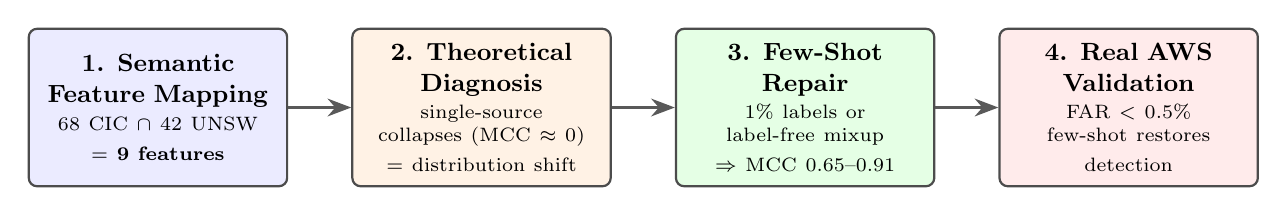
\begin{tikzpicture}[
  font=\small,
  >={Stealth[length=3mm]},
  box/.style={rounded corners=3pt, draw=black!70, line width=0.8pt,
              align=center, minimum height=20mm, text width=30mm, inner sep=4pt},
  s1/.style={box, fill=blue!8}, s2/.style={box, fill=orange!10},
  s3/.style={box, fill=green!10}, s4/.style={box, fill=red!8},
  arr/.style={->, line width=1.1pt, draw=black!65},
]
\node[s1] (sfm) at (0,0) {\textbf{1. Semantic\\Feature Mapping}\\[2pt]
  \scriptsize 68 CIC $\cap$ 42 UNSW\\ $=$ \textbf{9 features}};
\node[s2, right=8mm of sfm] (diag) {\textbf{2. Theoretical\\Diagnosis}\\[2pt]
  \scriptsize single-source\\ collapses (MCC $\approx$ 0)\\ = distribution shift};
\node[s3, right=8mm of diag] (fs) {\textbf{3. Few-Shot\\Repair}\\[2pt]
  \scriptsize 1\% labels or\\ label-free mixup\\ $\Rightarrow$ MCC 0.65--0.91};
\node[s4, right=8mm of fs] (aws) {\textbf{4. Real AWS\\Validation}\\[2pt]
  \scriptsize FAR $<$ 0.5\%\\ few-shot restores\\ detection};
\draw[arr] (sfm) -- (diag);
\draw[arr] (diag) -- (fs);
\draw[arr] (fs) -- (aws);
\end{tikzpicture}
}
% \end{graphicalabstract}

\begin{abstract}
Machine-learning-based network intrusion detection systems (NIDS) attain
near-perfect accuracy when trained and tested on the same network, yet their
ability to generalize across networks is rarely evaluated systematically. The
contribution of this paper is \emph{not} another off-the-shelf classifier on a
benchmark, but a \emph{methodology} for diagnosing and repairing cross-network
generalization, together with its validation on real cloud traffic. This paper
investigates two intertwined problems in practical NIDS: (1) the failure to
generalize across networks, and (2) \emph{feature-extractor mismatch} --- the
often-overlooked but operationally common situation where the same nominal feature
is computed differently by different flow-export tools (e.g., CICFlowMeter vs.\
Argus/Bro), a real obstacle whenever a model trained on one tool's output is
deployed behind another. Using a deliberately cross-source dataset pair ---
CSE-CIC-IDS2018 (68 features, CICFlowMeter) and UNSW-NB15 (42 features, Argus/Bro)
--- we construct a statistically validated \emph{Semantic Feature Mapping} (SFM)
that yields a truly comparable intersection feature set and, in the process,
exposes a concrete extractor mismatch on the TCP-window features (continuous in
CICFlowMeter, effectively binary in Argus/Bro) that we discard rather than
fabricate an equivalence. A single XGBoost model is used only as a
\emph{controlled backbone} to isolate the effect of the methodology, not as the
contribution. We find that a single XGBoost model
excelling in-domain (MCC $0.91$ on CIC; $0.74$ on UNSW) \emph{collapses}
cross-network (MCC $\approx 0$). Through controlled experiments we show that
(i) joint training shows that the nine SFM features carry \emph{sufficient
discriminative information} for both domains --- so the single-source failure
cannot be explained by a lack of discriminative information in the shared feature
space alone --- while the combined evidence identifies a directly measured
\emph{distribution shift} (large inter-domain Wasserstein distance and a
$\approx 0.99$ domain-classifier accuracy) as the \emph{major contributor}, with
class-conditional and label-taxonomy differences documented as additional factors
via a multi-class experiment; and (ii) minimal calibration --- only $1\%$ of
target-network labels, or supervised cross-dataset \emph{mixup} that uses only
target \emph{train} labels --- recovers cross-network MCC to the $0.65$--$0.91$
range. We validate these findings on real AWS cloud traffic: zero-shot deployment
fails (MCC $\approx 0$) but few-shot calibration with a small amount of domain
labels restores detection, although a stricter episode-level split shows that the
magnitude of the field benefit depends on the attack episode and the evaluation
protocol. As a complementary extension, we also classify attack \emph{categories}
(multi-class) on the same nine features, and show that the same per-category shift
that hurts binary transfer also limits multi-class cross-network transfer. All
numbers are drawn from real, reproducible experiments, providing deployment-oriented
evidence for designing and evaluating cross-network NIDS under distribution shift.
\end{abstract}

\begin{keyword}
network intrusion detection \sep cross-network generalization \sep semantic
feature mapping \sep domain adaptation \sep few-shot learning \sep XGBoost
\end{keyword}

\end{frontmatter}

% ============================================================
\section{Introduction}
\label{sec:intro}

Cyberattacks impose global economic losses estimated at around one trillion US
dollars in 2020 --- more than a $50\%$ increase since 2018
\citep{cremer} --- making machine-learning (ML) based network intrusion detection
systems (NIDS) an increasingly critical line of defense
\citep{torres,sarker,khraisat,buczak,bhuyan}. For two decades the research
community has evaluated NIDS on successive public benchmark datasets updated to
chase realism: from KDD~Cup~99 \citep{kdd} and NSL-KDD, to UNSW-NB15
\citep{unsw,unsweval} and CIC-IDS2017/CSE-CIC-IDS2018 \citep{cicids}, and more
recent variants for IoT and DDoS environments
\citep{botiot,toniot,ciciot,cicddos,ring}. On these datasets, reported accuracy
increasingly approaches perfection --- often exceeding $99\%$ across metrics
\citep{layeghy}. Yet this near-perfect academic performance has never truly
materialized as a comparable, practical NIDS in real production networks.

The gap between benchmark promise and deployment reality is rooted in a rarely
tested assumption: that training and operational data come from the same
distribution. Recent evidence suggests otherwise. \citet{layeghy} compared the
statistical distributions of benign traffic from three synthetic datasets
(UNSW-NB15, CIC-IDS2017, ToN-IoT) against two real production networks, and found
that the Wasserstein distance \citep{wasserstein} between the synthetic and
real-world groups is far larger than within-group distance --- for instance, the
mean packet inter-arrival time of benign UNSW-NB15 traffic is only
$\sim$\SI{0.02}{\second} while a real ISP network reaches
$\sim$\SI{2.28}{\second}. In terms of classification performance, \citet{cantone}
systematically measured the cross-dataset drop: the average Matthews Correlation
Coefficient (MCC) plummets from $0.946$ (within-dataset) to only $0.294$
(cross-dataset) --- effectively random guessing. These studies
\citep{cantone,layeghy,dhooge,verkerken} confirm the problem, but generally stop
at \emph{observing} the drop: they rarely disentangle feature insufficiency from
distribution shift, nor offer a low-cost, controlled-validated solution. We take a
step toward this by ruling out feature insufficiency and directly measuring the
distribution shift, and by documenting label-taxonomy differences through a
multi-class experiment.

This paper is a direct continuation of our prior NIDS work on CSE-CIC-IDS2018
(XGBoost \citep{xgboost} feature reduction plus real-traffic AWS validation), which
explicitly acknowledged its limitations. Two of these limitations form the
\textbf{core gaps} of this paper:
\begin{enumerate}
  \item \textbf{Cross-network generalization failure.} Models collapse when facing
  traffic characteristics from a different network topology.
  \item \textbf{Feature-extractor mismatch.} Differing feature definitions across
  extraction tools (CICFlowMeter vs Argus/Bro) degrade accuracy at real inference.
\end{enumerate}

\paragraph{Contributions.} The contributions of this paper are:
\begin{itemize}
  \item A cross-dataset, statistically validated \textbf{Semantic Feature Mapping
  (SFM)}, including a \emph{feature-extractor mismatch} finding on TCP-window
  features (Section~\ref{sec:sfm}).
  \item \textbf{Quantitative evidence} that single-source NIDS collapse
  cross-network (Section~\ref{sec:baseline}).
  \item A \textbf{diagnosis} showing --- via joint training --- that the shared
  features carry sufficient discriminative information for both domains (so feature
  insufficiency is not the sole explanation), and identifying a directly measured
  \emph{distribution shift} as the \emph{major contributor} to the cross-network gap
  (with class-conditional/taxonomy differences acknowledged as additional factors),
  together with \textbf{low-cost solutions}: minimal $1\%$ target-label calibration,
  or cross-dataset \emph{mixup} (Sections~\ref{sec:align},~\ref{sec:da}).
  \item \textbf{Real-traffic validation} on cloud infrastructure (AWS): measuring
  False Alarm Rate, quantitatively diagnosing three-domain \emph{distribution
  shift}, and restoring detection via \emph{few-shot} calibration
  (Section~\ref{sec:realtraffic}).
  \item A \textbf{multi-class extension} that classifies attack \emph{categories}
  on the same nine SFM features, reporting in-domain per-category performance and
  showing that the same per-category shift limits multi-class cross-network
  transfer (Section~\ref{sec:multiclass}).
\end{itemize}

\paragraph{Positioning and novelty.} We stress that this work is \emph{not} the
routine application of an existing classifier to a standard dataset. The novelty
lies in the methodology --- a statistically validated cross-tool feature mapping,
a controlled diagnosis that shows the shared features are sufficiently informative
(so feature insufficiency is not the sole explanation) and isolates a directly
measured distribution shift as the major contributor (conceptually
motivated by the Ben-David bound), and an end-to-end validation on real cloud
traffic including False Alarm Rate, a quantified three-domain distribution shift,
and few-shot repair. XGBoost is deliberately fixed as a lightweight, reproducible
backbone precisely so that any measured effect is attributable to the methodology
rather than to model capacity; the security contribution is the transferable
recipe for making a single-source NIDS work on a previously unseen network at
minimal labeling cost.

\paragraph{Research questions.} This paper addresses five research questions.
\textbf{RQ1:} can semantically equivalent flow features extracted by heterogeneous
tools be reliably identified for cross-network NIDS? \textbf{RQ2:} to what extent
does a single-source NIDS generalize to an unseen network after semantic feature
alignment? \textbf{RQ3:} what evidence distinguishes representation insufficiency
from distribution shift as contributors to cross-network degradation? \textbf{RQ4:}
how much target-domain labeling is required to recover cross-network detection
performance? \textbf{RQ5:} does the adaptation strategy transfer from benchmark
datasets to real AWS traffic?

\paragraph{Experimental transparency and reproducibility.} All reported values are
obtained from executed experiments; no illustrative values are presented as
empirical results, and negative or non-monotone outcomes are reported as observed.

% ============================================================
\section{Related Work}
\label{sec:related}

\paragraph{ML-based NIDS.} Tree-based models (e.g., XGBoost
\citep{xgboost,husain,zhou}) and deep neural networks
\citep{shone,liulang,mahdavifar,wu,duan} are widely used on benchmark datasets
\citep{unsw,cicids}. Most report high in-domain results (train/test on the same
dataset), but this does not guarantee robustness on traffic differing from the
training data. We deliberately choose XGBoost for its efficiency, its handling of
imbalanced tabular data, and its light resource footprint --- properties relevant
to \emph{edge} deployment.

\paragraph{Cross-dataset generalization.} Several studies measure how poorly NIDS
generalize across networks. \citet{dhooge} evaluated many supervised classifiers
across CIC-IDS2017 and CSE-CIC-IDS2018 and concluded that models fail on networks
unseen during training. \citet{verkerken} reported an average AUROC drop of
$30.45\%$ in cross-dataset experiments with unsupervised models. \citet{cantone}
extended the analysis to four datasets and documented MCC falling from $0.946$
(within) to $0.294$ (cross), while showing that a few features often suffice to
separate classes \emph{within} a single dataset --- a symptom of dataset-specific
over-correlation that harms generalization. To standardize comparison,
\citet{sarhan,sarhannf} proposed a unified NetFlow feature set. These works confirm
the problem but stop at observing the drop --- without separating the contribution
of \emph{feature insufficiency} versus \emph{distribution shift}, and without
offering low-cost recovery. Our paper narrows this gap: a controlled diagnosis that
shows the shared features are sufficiently informative (so feature insufficiency is
not the sole explanation) and directly measures the distribution shift (with
label-taxonomy differences documented through a multi-class experiment), plus a
minimal-calibration solution.

\paragraph{Dataset integrity and realism.} Part of the cross-dataset drop stems
from flaws in dataset construction itself. \citet{engelen} reconstructed
CIC-IDS2017 and found over $20\%$ of flows needed fixing/relabeling; \citet{rosay}
identified feature duplication, miscomputation, and protocol-detection errors in
CICFlowMeter (echoed by \citet{lanvin}); while \citet{liu} reported labeling error
rates of $6.67\%$ and $7.53\%$ on CIC-IDS2017 and CSE-CIC-IDS2018 respectively.
\citet{catillo} even questioned whether NIDS progress on public datasets reflects
real advances or academic hype. Complementarily, \citet{layeghy} showed that the
statistical distributions of synthetic benign traffic differ significantly (large
Wasserstein distance) from real production networks, questioning how far
synthetic-trained models transfer. These findings motivate us to (i) build a
semantically comparable feature mapping across extraction tools, and (ii) validate
the model on real traffic (Section~\ref{sec:conclusion}).

\paragraph{Domain adaptation and collaborative learning.} CORAL \citep{coral}
aligns second-order statistics (covariance) across domains, while MMD-based
approaches align distribution moments; their application and evaluation on
network \emph{tabular} data remain limited. \emph{Few-shot} approaches have also
begun to be explored for label-limited NIDS \citep{fewshot}. As an alternative,
\emph{federated learning} seeks to improve generalization by training a global
model across organizations without sharing raw data
\citep{nidsfgpa,popoola,bertoli,agrawal}, although the model typically remains
exposed to data from all sources at evaluation, which can bias the measurement of
true generalization \citep{cantone}. We evaluate CORAL, joint training,
\emph{few-shot}, and cross-dataset \emph{mixup} directly on the CIC-IDS2018 and
UNSW-NB15 pair.

\paragraph{Why not deep domain adaptation?} More expressive deep domain-adaptation
methods --- e.g., Deep CORAL and adversarial alignment such as DANN --- can, in
principle, learn non-linear domain-invariant representations. We deliberately do
not adopt them here for three reasons aligned with our edge-deployment target.
(i) \emph{Cost.} DANN and Deep CORAL require training a deep feature extractor
(and, for DANN, an adversarial domain discriminator), incurring memory, compute,
and energy budgets that are impractical for smart routers, IoT gateways, or inline
sensors, and inference latency that may exceed the flow arrival rate --- precisely
what our single, $2.9$~MB, sub-millisecond XGBoost avoids. (ii) \emph{Data regime.}
Deep alignment typically needs large volumes of (unlabeled) target data to
estimate stable invariant representations; our premise is the opposite --- a new
network offers little target data, which is exactly where a few labeled anchors
(few-shot) are more data-efficient. (iii) \emph{Tabular mismatch.} On tabular
flow features, tree ensembles remain strong and stable, while adversarial
alignment is notoriously unstable to train and offers limited gains over simpler
statistics-matching on this data type. We therefore treat deep DA as a
complementary, heavier-weight alternative rather than a baseline for the
edge-constrained regime studied here. In particular, domain-invariant NIDS such as
the DI-NIDS line of work \citep{layeghy}, which learns invariant representations to
close the synthetic-to-real gap, is conceptually the closest heavyweight
counterpart to our lightweight recipe; a controlled head-to-head comparison
(accuracy, label budget, and edge cost) against DI-NIDS and adversarial
domain-adaptation baselines is an important direction that we leave to future work,
since it requires a different (deep) training and evaluation stack than the
reproducible XGBoost backbone deliberately fixed here. We make this scope
limitation explicit rather than claim superiority we have not measured.

% ============================================================
\section{Data and Semantic Feature Mapping}
\label{sec:sfm}

\subsection{Datasets}
We use a deliberately \emph{cross-source} pair:
\begin{itemize}
  \item \textbf{CSE-CIC-IDS2018}: CIC testbed traffic (2018), extracted with
  CICFlowMeter, 68 clean features. Multi-class labels (Benign + 14 attack types);
  for this stage collapsed to binary (attack/normal).
  \item \textbf{UNSW-NB15}: traffic generated by IXIA PerfectStorm (2015),
  extracted with Argus \& Bro/Zeek, 42 features, 10 classes. Partition files:
  $175{,}341$ records (used as training data) and $82{,}332$ records (test data).
\end{itemize}
This difference in extraction tools and traffic sources is not a weakness but a
prerequisite for realistically testing the core gaps.

\paragraph{Multi-class attack composition.} Although the detection task in this
paper is binary, both datasets retain their original attack taxonomy (CIC labels
are preserved in the raw CSV; UNSW provides \texttt{attack\_cat}). We report the
per-category composition of the \emph{attack} population in
Table~\ref{tab:attackcomp} and Figure~\ref{fig:attackcomp} to make the
class-imbalance across attack types explicit. Both datasets are dominated by a few
categories --- CIC by DDoS ($46.0\%$) and DoS ($23.8\%$), UNSW by Generic
($41.7\%$) and Exploits ($24.6\%$) --- while minority types (UNSW Analysis,
Backdoor, Shellcode) each account for $<1.5\%$. This steep per-category imbalance
is precisely why a uniform $1\%$ few-shot budget would leave rare categories with
too few samples for reliable multi-class adaptation (Section~\ref{sec:conclusion}).

\begin{table}[h]
\centering
\caption{Initial multi-class attack-label composition (attack flows only, real
counts from the sampled populations). CIC categories group the original 2018 labels
(e.g., DoS = Hulk/GoldenEye/Slowloris/SlowHTTPTest); UNSW uses \texttt{attack\_cat}.}
\label{tab:attackcomp}
\small
\begin{tabular}{lr r @{\hskip 2em} lr r}
\toprule
\multicolumn{3}{c}{CSE-CIC-IDS2018} & \multicolumn{3}{c}{UNSW-NB15} \\
\cmidrule(lr){1-3}\cmidrule(lr){4-6}
Category & $n$ & \% & Category & $n$ & \% \\
\midrule
DDoS         & $126{,}389$ & $46.0$ & Generic   & $18{,}860$ & $41.7$ \\
DoS          & $65{,}426$  & $23.8$ & Exploits  & $11{,}125$ & $24.6$ \\
BruteForce   & $38{,}174$  & $13.9$ & Fuzzers   & $6{,}048$  & $13.4$ \\
Botnet       & $28{,}618$  & $10.4$ & DoS       & $4{,}086$  & $9.0$  \\
Infiltration & $16{,}047$  & $5.8$  & Recon     & $3{,}494$  & $7.7$  \\
             &             &        & Analysis  & $677$      & $1.5$  \\
             &             &        & Backdoor  & $583$      & $1.3$  \\
             &             &        & Shellcode & $378$      & $0.8$  \\
\midrule
Total attack & $274{,}654$ & $100$ & Total attack & $45{,}251$ & $100$ \\
\bottomrule
\end{tabular}
\end{table}

\begin{figure}[h]
\centering
\resizebox{0.95\linewidth}{!}{% TikZ-only (input-able) pie charts of attack composition. Requires: \usepackage{tikz}
\begin{tikzpicture}[font=\footnotesize]
\def\R{2.2}
\newcommand{\wedge}[4]{% center-x, start, end, color
  \fill[#4] (#1,0) -- ++(#2:\R) arc (#2:#3:\R) -- cycle;
  \draw[white,line width=0.6pt] (#1,0) -- ++(#2:\R);}
\newcommand{\lgd}[3]{\fill[#3] (#1,#2) rectangle ++(0.28,0.28);}

% CIC (left)
\begin{scope}[shift={(0,0)}]
  \node[font=\bfseries] at (0,2.9) {CSE-CIC-IDS2018 (attack flows)};
  \wedge{0}{0}{165.66}{blue!55}
  \wedge{0}{165.66}{251.42}{orange!70}
  \wedge{0}{251.42}{301.46}{green!55!black}
  \wedge{0}{301.46}{338.97}{red!60}
  \wedge{0}{338.97}{360}{purple!55}
  \begin{scope}[shift={(-1.1,-3.4)}]
    \lgd{0}{0}{blue!55} \node[anchor=west] at (0.34,0.14){DDoS 46.0\%};
    \lgd{0}{-0.42}{orange!70} \node[anchor=west] at (0.34,-0.28){DoS 23.8\%};
    \lgd{0}{-0.84}{green!55!black} \node[anchor=west] at (0.34,-0.70){Brute-Force 13.9\%};
    \lgd{2.4}{0}{red!60} \node[anchor=west] at (2.74,0.14){Botnet 10.4\%};
    \lgd{2.4}{-0.42}{purple!55} \node[anchor=west] at (2.74,-0.28){Infiltration 5.8\%};
  \end{scope}
\end{scope}

% UNSW (right)
\begin{scope}[shift={(7.4,0)}]
  \node[font=\bfseries] at (0,2.9) {UNSW-NB15 (attack flows)};
  \wedge{0}{0}{150.04}{blue!55}
  \wedge{0}{150.04}{238.55}{orange!70}
  \wedge{0}{238.55}{286.67}{green!55!black}
  \wedge{0}{286.67}{319.17}{red!60}
  \wedge{0}{319.17}{346.97}{purple!55}
  \wedge{0}{346.97}{352.35}{brown!60}
  \wedge{0}{352.35}{356.99}{teal!60}
  \wedge{0}{356.99}{360}{gray!60}
  \begin{scope}[shift={(-1.1,-3.4)}]
    \lgd{0}{0}{blue!55} \node[anchor=west] at (0.34,0.14){Generic 41.7\%};
    \lgd{0}{-0.42}{orange!70} \node[anchor=west] at (0.34,-0.28){Exploits 24.6\%};
    \lgd{0}{-0.84}{green!55!black} \node[anchor=west] at (0.34,-0.70){Fuzzers 13.4\%};
    \lgd{0}{-1.26}{red!60} \node[anchor=west] at (0.34,-1.12){DoS 9.0\%};
    \lgd{2.4}{0}{purple!55} \node[anchor=west] at (2.74,0.14){Recon 7.7\%};
    \lgd{2.4}{-0.42}{brown!60} \node[anchor=west] at (2.74,-0.28){Analysis 1.5\%};
    \lgd{2.4}{-0.84}{teal!60} \node[anchor=west] at (2.74,-0.70){Backdoor 1.3\%};
    \lgd{2.4}{-1.26}{gray!60} \node[anchor=west] at (2.74,-1.12){Shellcode 0.8\%};
  \end{scope}
\end{scope}
\end{tikzpicture}
}
\caption{Initial multi-class attack composition per dataset. Both are dominated by
a few high-volume categories, with a long tail of minority attack types --- a steep
per-category imbalance relevant to multi-class few-shot adaptation.}
\label{fig:attackcomp}
\end{figure}

\subsection{Mapping Construction and Validation}
\label{sec:sfmmap}
SFM maps functionally equivalent features across datasets even when column names
differ (e.g., \texttt{Flow Duration}$\leftrightarrow$\texttt{dur}). Because the
extraction tools differ (CICFlowMeter vs Argus/Bro), each candidate pair is
\emph{not} accepted based on name similarity, but \emph{statistically validated}
in three steps: (i) matching feature semantics from each tool's official
documentation; (ii) returning CIC features to their original scale
($x_{\text{orig}} = x_{\text{scaled}}\cdot\sigma + \mu$, since our CIC release is
already z-scored); and (iii) comparing summary statistics (median, 99th
percentile, maximum) of each pair to assess \emph{scale-order} equivalence. A pair
is deemed \emph{aligned} when the median and p99 ratios lie in the same order of
magnitude; \emph{scale-mismatch} when they differ by $1$--$3$ orders (unit
conversion needed); and \emph{different-feature} when $>3$ orders.

Table~\ref{tab:sfm} summarizes the mapping. Nine pairs qualify as the strong
intersection (Model~A), two IAT pairs are kept as an optional add-on (Model~B),
and two ``TCP window'' pairs are \emph{discarded} because they prove
non-comparable despite similar names.

\begin{table*}[t]
\centering
\caption{Semantic Feature Mapping (SFM) CSE-CIC-IDS2018 $\leftrightarrow$
UNSW-NB15, statistically validated on the \emph{original scale} (CIC un-scaled
first). Median columns show the order of magnitude in each dataset; the
\emph{note} column summarizes the comparability verdict. The top nine pairs form
\textbf{Model~A}; two IAT pairs are added in \textbf{Model~B}. Two TCP-window
pairs are discarded as \emph{feature-extractor mismatch}. Scale/unit differences
are resolved by per-dataset \emph{z-score} normalization, so pairs remain
\emph{semantically comparable} even when medians differ by orders of magnitude.}
\label{tab:sfm}
\small
\begin{tabular}{lllrrl}
\toprule
CIC feature & UNSW feature & Meaning & CIC median & UNSW median & Comparability note \\
\midrule
\texttt{Flow Duration}     & \texttt{dur}    & Flow duration & $20761$ & $0.0016$ & Model A; unit diff ($\mu$s vs s) \\
\texttt{Tot Fwd Pkts}      & \texttt{spkts}  & Forward packets  & $2$ & $2$ & Model A; aligned \\
\texttt{Tot Bwd Pkts}      & \texttt{dpkts}  & Backward packets & $1$ & $2$ & Model A; same order \\
\texttt{TotLen Fwd Pkts}   & \texttt{sbytes} & Forward bytes    & $43$ & $430$ & Model A; comparable order \\
\texttt{TotLen Bwd Pkts}   & \texttt{dbytes} & Backward bytes   & $101$ & $164$ & Model A; aligned \\
\texttt{Fwd Pkt Len Mean}  & \texttt{smean}  & Mean fwd pkt size & $36$ & $73$ & Model A; aligned \\
\texttt{Bwd Pkt Len Mean}  & \texttt{dmean}  & Mean bwd pkt size & $66$ & $44$ & Model A; aligned \\
\texttt{Flow Byts/s}       & \texttt{sload}  & Source byte rate  & $787.5$ & $8.80{\times}10^{5}$ & Model A; unit diff (byte/s vs bit/s)$^\dagger$ \\
\texttt{Bwd Pkts/s}        & \texttt{dload}  & Dest.\ packet rate & $3.70$ & $1447$ & Model A; unit diff (pkt/s vs bit/s)$^\dagger$ \\
\midrule
\texttt{Fwd IAT Mean}      & \texttt{sinpkt} & Fwd inter-arrival & $3544$ & $0.28$ & Model B; unit diff ($\mu$s vs ms) \\
\texttt{Bwd IAT Mean}      & \texttt{dinpkt} & Bwd inter-arrival & $0$ & $0.006$ & Model B; optional \\
\midrule
\texttt{Init Fwd Win Byts} & \texttt{swin}   & TCP window (fwd)  & $953$ & $0$ & \emph{Discarded}: UNSW binary $\{0,255\}$ vs CIC continuous \\
\texttt{Init Bwd Win Byts} & \texttt{dwin}   & TCP window (bwd)  & $-1$ & $0$ & \emph{Discarded}: UNSW binary $\{0,255\}$ vs CIC continuous \\
\bottomrule
\end{tabular}

\vspace{0.4em}
\raggedright{\footnotesize $^\dagger$Rate features: UNSW \texttt{sload}/\texttt{dload}
are reported by Argus in \emph{bits/second}; CIC \texttt{Flow Byts/s} is in
\emph{bytes/second} and \texttt{Bwd Pkts/s} in \emph{packets/second}. This unit
mismatch is explicitly corrected in the real-traffic validation
(Section~\ref{sec:rt-shift}). UNSW medians are computed on the $175{,}341$-record
training file; CIC medians on values returned to the original scale.}
\end{table*}

\paragraph{Key finding: TCP-window mismatch.} Unique-value inspection proves that
\texttt{swin}/\texttt{dwin} in UNSW are practically binary ($\{0, 255\}$), whereas
\texttt{Init Fwd/Bwd Win Byts} in CIC are continuous ($0$--$65535$). Although the
official descriptions call both ``TCP window,'' the data are not comparable. We
\emph{discard} this pair and report it as a case study of \emph{feature-extractor
mismatch} (gap \#2). This case underscores the importance of statistical
validation: without distribution inspection, these similarly named pairs would
pass and inject cross-network noise.

\subsection{Final Feature Set and Preprocessing}
We apply StandardScaler (z-score) \emph{per dataset separately} so that
unit/scale differences are normalized without fabricating conversions. The final
features (\textbf{Model~A}, 9 strong intersection features): \texttt{dur, spkts,
dpkts, sbytes, dbytes, smean, dmean, sload, dload}. \textbf{Model~B} adds
\texttt{sinpkt, dinpkt} (Fwd/Bwd IAT). Model~A is the basis because it matches
Model~B while being more compact.

\paragraph{No data leakage in scaling.} To avoid any train--test contamination,
the scaler statistics (per-feature mean $\mu$ and standard deviation $\sigma$) are
estimated \emph{exclusively on the training set} and then \emph{applied} (transform
only) to the held-out test set and to the AWS traffic; that is, we call
\texttt{fit} on train and \texttt{transform} on evaluation data --- never
\texttt{fit\_transform} on the union. In the few-shot setting, when a small
fraction of target labels is added to training, $\mu,\sigma$ are re-estimated on
that augmented training set only, and the fixed target test set remains untouched.
The Wasserstein analysis (Section~\ref{sec:wass}) likewise fits its $z$-space on
the target \emph{train} set alone. This guarantees that no test-time information
influences either scaling or model selection. Figure~\ref{fig:unscaling}
illustrates the full cross-extractor pipeline: un-scaling to original units,
comparison on the original scale to derive the SFM verdict, and per-dataset
re-$z$-scoring fitted on training data only.

\begin{figure}[h]
\centering
\resizebox{0.95\linewidth}{!}{% TikZ-only (input-able). Requires: \usepackage{tikz}\usetikzlibrary{arrows.meta,positioning}
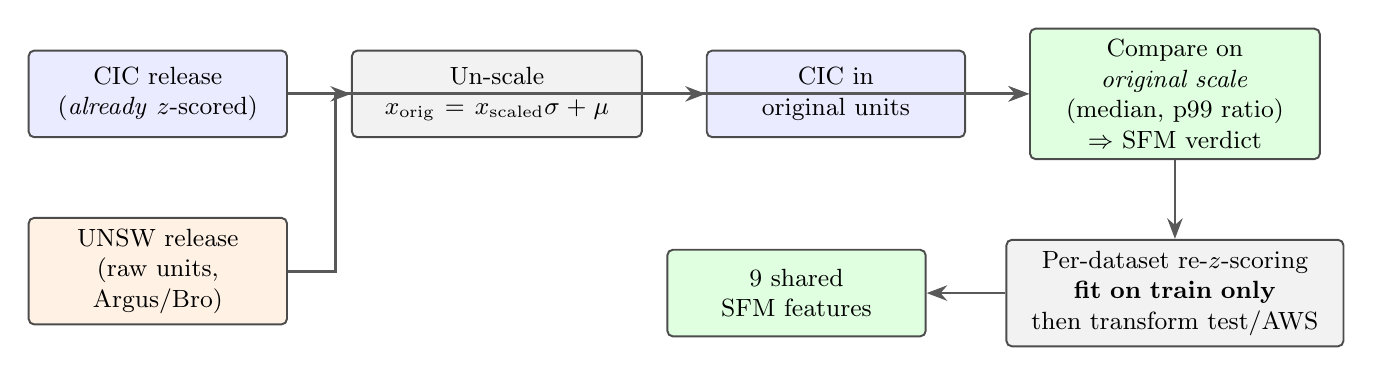
\begin{tikzpicture}[
  font=\small, >={Stealth[length=2.6mm]},
  b/.style={rounded corners=2pt, draw=black!70, line width=0.7pt, align=center,
            inner sep=4pt, minimum height=11mm, text width=30mm},
  cic/.style={b, fill=blue!8}, uns/.style={b, fill=orange!10},
  op/.style={b, fill=black!5, text width=34mm}, shared/.style={b, fill=green!12, text width=34mm},
  a/.style={->, line width=1pt, draw=black!65},
]
\node[cic] (cicz) {CIC release\\(\emph{already} $z$-scored)};
\node[op, right=8mm of cicz] (uns1) {Un-scale\\$x_{\text{orig}}=x_{\text{scaled}}\sigma+\mu$};
\node[cic, right=8mm of uns1] (cico) {CIC in\\original units};
\node[uns, below=10mm of cicz] (unsraw) {UNSW release\\(raw units,\\Argus/Bro)};
\node[shared, right=8mm of cico] (cmp) {Compare on\\\emph{original scale}\\(median, p99 ratio)\\$\Rightarrow$ SFM verdict};
\node[op, below=10mm of cmp, text width=40mm] (rez)
  {Per-dataset re-$z$-scoring\\\textbf{fit on train only}\\then transform test/AWS};
\node[shared, left=10mm of rez, text width=30mm] (model) {9 shared\\SFM features};
\draw[a] (cicz) -- (uns1);
\draw[a] (uns1) -- (cico);
\draw[a] (cico) -- (cmp);
\draw[a] (unsraw.east) -- ++(0.6,0) |- (cmp.west);
\draw[a] (cmp) -- (rez);
\draw[a] (rez) -- (model);
\end{tikzpicture}
}
\caption{Cross-extractor alignment for SFM. CIC features are un-scaled to their
original units, compared with raw UNSW on the original scale (median/p99 ratios) to
assign the comparability verdict, then both datasets are independently
$z$-scored with statistics fitted \emph{only} on their training partitions
(no leakage into test/AWS).}
\label{fig:unscaling}
\end{figure}

\subsection{Model Selection and Deployment Efficiency}
\label{sec:edge}
We deliberately keep a \textbf{single XGBoost model} rather than a heavy ensemble
or complex deep learning. Besides preserving comparability with prior work and
isolating the contributing variable (SFM and cross-network adaptation, not model
capacity), this choice aligns with \textbf{edge deployment} needs and low
computational footprint. On real edge devices --- smart routers, IoT
gateways, or inline sensors --- multi-algorithm ensembles or large deep networks
are unrealistic due to high memory, CPU, and energy consumption, and inference
latency that may exceed the flow arrival rate. In contrast, a single XGBoost with
$9$ features yields a light binary model and fast tree-based inference, making it
an \emph{edge-friendly} NIDS candidate.

\begin{table}[h]
\centering
\caption{Efficiency profile of Model~A (9 features), measured on a single CPU
core (single-thread, emulating a 1-vCPU edge).}
\label{tab:efficiency}
\begin{tabular}{lc}
\toprule
Metric & Value \\
\midrule
Binary model size (Model A, 9 features, 200 trees) & $2.9$ MB \\
Mean inference latency per flow (batch$=1$) & $\approx 439\ \mu$s \\
Inference throughput (1 vCPU, incremental) & $\approx 2{,}276$ flows/s \\
\bottomrule
\end{tabular}
\end{table}

\noindent The figures in Table~\ref{tab:efficiency} come from real measurements
(single-thread XGBoost, batch$=1$; median $434\ \mu$s, std $23\ \mu$s over
$\sim$2000 flows). The $2.9$ MB model (200 trees, depth 8) is compact enough for
edge devices, and $>2{,}000$ flows/s per core suffices for many network monitoring
points, supporting suitability for resource-constrained edge deployment. We report
latency in the hundreds of microseconds (not tens), and avoid reporting batch
throughput that could mislead via vectorization gains.

\paragraph{Deployment context and scalability.} The $\approx 2{,}276$ flows/s on a
\emph{single} core is intended for edge/branch scenarios --- smart routers, IoT
gateways, or border CPE --- handling moderate flow aggregates, not a high-speed
core network. For line-rate traffic (e.g., $10$ Gbps reaching tens of thousands of
flows/s), XGBoost inference is \emph{embarrassingly parallel} at the flow level:
each flow is scored independently, so multi-thread processing on $8$--$16$ core
CPUs scales throughput near-linearly to $\approx 18{,}000$--$35{,}000$ flows/s ---
adequate for line-rate monitoring --- without changing the model. In other words,
the single-core figure is a conservative per-core lower bound, not a system
ceiling.

% ============================================================
\section{Cross-Dataset Baseline: The Generalization Gap}
\label{sec:baseline}

We train XGBoost (\texttt{max\_depth}=8, \texttt{lr}=0.1,
\texttt{n\_estimators}=200, \texttt{subsample}/\texttt{colsample}=0.8) and evaluate
four scenarios using scikit-learn \citep{sklearn} with stratified train/test
splits \citep{kohavi}. The primary metric is the Matthews Correlation Coefficient
(MCC) \citep{matthews,chicco}, more informative and robust to class imbalance than
accuracy.

Label verification was performed: on CIC \texttt{Benign}$=0$; the binary
conversion yields exactly $1{,}348{,}453$ normal and $274{,}808$ attack, so the
negative cross-network MCC is a genuine phenomenon, not a labeling artifact.

\begin{table}[h]
\centering
\caption{Cross-dataset baseline (MCC, Model A). High in-domain performance
collapses cross-network.}
\label{tab:baseline}
\begin{tabular}{lcc}
\toprule
Scenario & Model A & Model B \\
\midrule
Same-CIC (train \& test CIC)   & $0.913$ & $0.914$ \\
Same-UNSW (train \& test UNSW) & $0.745$ & $0.743$ \\
CIC$\rightarrow$UNSW          & $-0.072$ & $0.004$ \\
UNSW$\rightarrow$CIC          & $-0.061$ & $-0.046$ \\
\midrule
\emph{Generalization gap}     & $0.81$--$0.99$ & $0.79$--$0.91$ \\
\bottomrule
\end{tabular}
\end{table}

\begin{figure}[h]
\centering
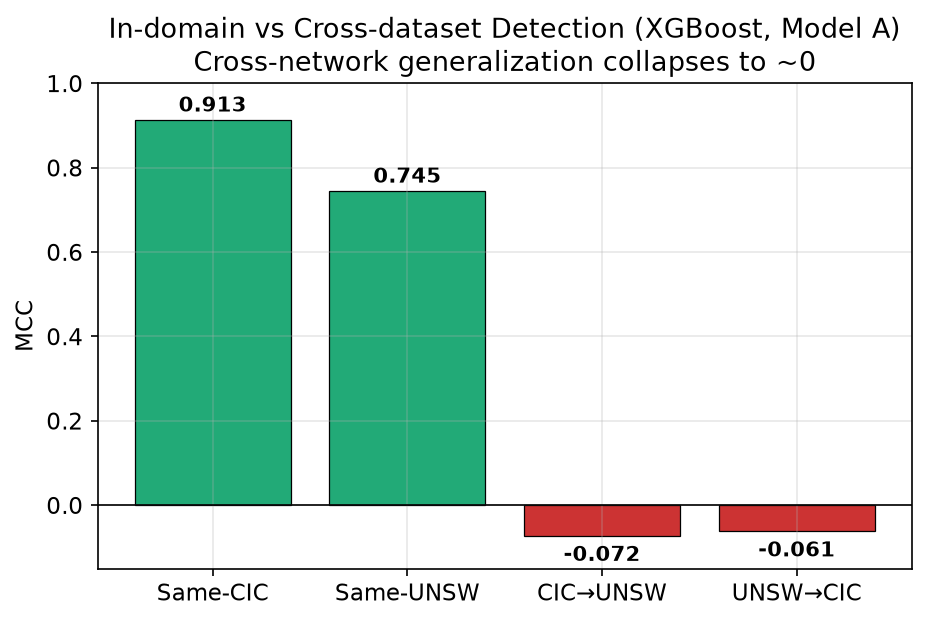
\includegraphics[width=0.72\linewidth]{fig1_generalization_gap.png}
\caption{In-domain vs cross-dataset detection. A model excelling in-domain falls
to MCC $\approx 0$ cross-network.}
\label{fig:gap}
\end{figure}

Table~\ref{tab:baseline} and Figure~\ref{fig:gap} show MCC $\approx 0$ (random
guessing) to negative cross-network. This is empirical evidence of gap \#1.

% ============================================================
\section{Diagnosis: The Gap Is Dominated by Distribution Shift}
\label{sec:align}

\paragraph{Conceptual motivation: the Ben-David domain-adaptation bound.} Before
the empirical evidence, we invoke a theoretical framework --- \emph{as a conceptual
motivation, not as an empirical decomposition of the bound} --- that helps explain
\emph{why} minimal calibration can recover performance. By the theory of
domain-adaptation generalization bounds \citep{bendavid}, the target-domain error
$R_T(h)$ is bounded by:
\begin{equation}
\label{eq:bendavid}
R_T(h) \;\le\; R_S(h) \;+\; \tfrac{1}{2}\, d_{\mathcal{H}\Delta\mathcal{H}}(\mathcal{D}_S, \mathcal{D}_T) \;+\; \lambda^\ast,
\end{equation}
where $R_S(h)$ is the source-domain error, $d_{\mathcal{H}\Delta\mathcal{H}}$ is
the source--target distribution \emph{discrepancy} defined on the hypothesis
space $\mathcal{H}$, and $\lambda^\ast$ is the ideal-joint error (the error of the
best classifier valid on both domains). We use this framework only to interpret
the \emph{qualitative} role of each component of our method, with three
qualifications we state explicitly to avoid overstating the theory: (i)
\textbf{SFM establishes a semantically comparable input representation across
domains} --- by equating feature definitions/units across extraction tools, SFM
makes cross-domain distribution comparison \emph{meaningful} and enables controlled
adaptation experiments; we do \emph{not} claim that SFM by itself aligns the
hypothesis space $\mathcal{H}$ or directly reduces $d_{\mathcal{H}\Delta\mathcal{H}}$;
(ii) we measure the input-distribution discrepancy only \emph{as a proxy}, via the
Wasserstein distance $W_1$ (Section~\ref{sec:wass}) and a domain classifier
(Section~\ref{sec:rt-shift}) --- $W_1$ is \textbf{not} equivalent to
$d_{\mathcal{H}\Delta\mathcal{H}}$ (the latter is defined over the hypothesis space
and is classifier-dependent), but a computable distributional distance that
indicates the magnitude of \emph{covariate shift}; (iii) $1\%$ few-shot and mixup
can be understood as providing information about the target ideal classifier
(related to $\lambda^\ast$) and shifting the training distribution toward the
target, and are thus \emph{conceptually} consistent with lowering the
right-hand terms of Eq.~\eqref{eq:bendavid}. We stress that the MCC recovery we
observe (Section~\ref{sec:da}) is \emph{empirical} evidence from controlled
experiments; the Ben-David framework motivates it rather than serving as a direct
measurement of the bound's terms. Figure~\ref{fig:bendavid} illustrates these
components schematically.

\begin{figure}[h]
\centering
\resizebox{0.9\linewidth}{!}{% TikZ-only (input-able). Requires: \usepackage{tikz}\usetikzlibrary{arrows.meta,positioning}
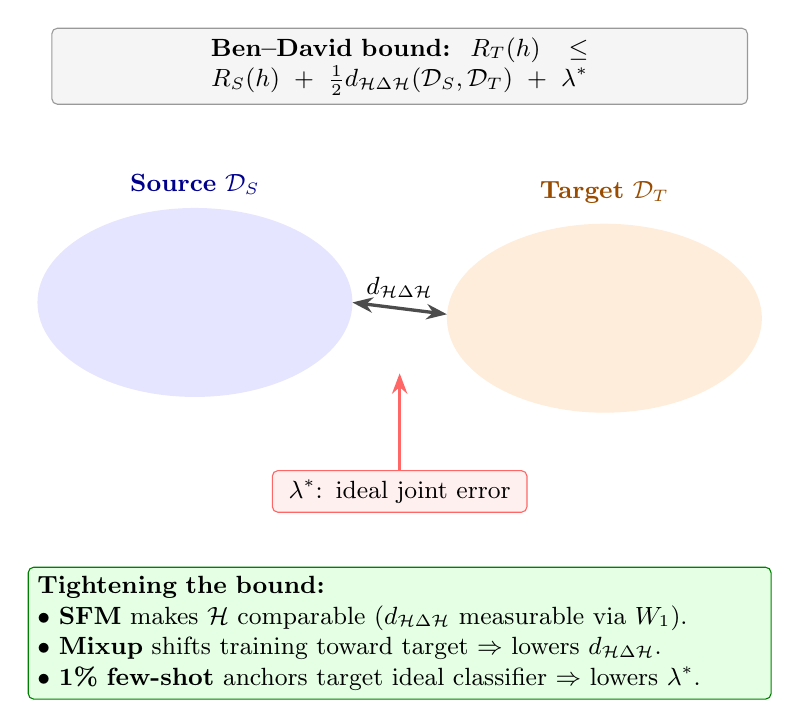
\begin{tikzpicture}[font=\small,>={Stealth[length=2.6mm]}]
  \fill[blue!10,rounded corners=10pt] (0,0) ellipse (2.0 and 1.2);
  \node[blue!55!black] at (0,1.5) {\textbf{Source} $\mathcal{D}_S$};
  \fill[orange!14,rounded corners=10pt] (5.2,-0.2) ellipse (2.0 and 1.2);
  \node[orange!60!black] at (5.2,1.4) {\textbf{Target} $\mathcal{D}_T$};
  \draw[<->,line width=1.2pt,draw=black!70] (2.0,0) -- (3.2,-0.15)
    node[midway,above,align=center]{$d_{\mathcal{H}\Delta\mathcal{H}}$};
  \node[draw=red!60,fill=red!6,rounded corners=2pt,align=center,text width=30mm]
    (lam) at (2.6,-2.4) {$\lambda^\ast$: ideal joint error};
  \draw[->,red!60,line width=0.9pt] (lam.north) -- (2.6,-0.9);
  \node[draw=black!40,fill=black!4,rounded corners=2pt,align=center,text width=86mm]
    (bound) at (2.6,3.0)
    {\textbf{Ben--David bound:}\;
     $R_T(h)\le R_S(h)+\tfrac12 d_{\mathcal{H}\Delta\mathcal{H}}(\mathcal{D}_S,\mathcal{D}_T)+\lambda^\ast$};
  \node[draw=green!50!black,fill=green!10,rounded corners=2pt,align=left,text width=92mm]
    (act) at (2.6,-4.2)
    {\textbf{Tightening the bound:}\\
     $\bullet$ \textbf{SFM} makes $\mathcal{H}$ comparable ($d_{\mathcal{H}\Delta\mathcal{H}}$ measurable via $W_1$).\\
     $\bullet$ \textbf{Mixup} shifts training toward target $\Rightarrow$ lowers $d_{\mathcal{H}\Delta\mathcal{H}}$.\\
     $\bullet$ \textbf{1\% few-shot} anchors target ideal classifier $\Rightarrow$ lowers $\lambda^\ast$.};
\end{tikzpicture}
}
\caption{Schematic (conceptual-motivation) view of the Ben--David bound. The source
($\mathcal{D}_S$) and target ($\mathcal{D}_T$) feature distributions are separated
by a discrepancy $d_{\mathcal{H}\Delta\mathcal{H}}$; $\lambda^\ast$ is the ideal
joint error. SFM provides a semantically comparable input representation (enabling
us to measure input-distribution distance via $W_1$ as a proxy --- $W_1$ is not
equal to $d_{\mathcal{H}\Delta\mathcal{H}}$); cross-dataset mixup shifts training
toward the target; and $1\%$ few-shot anchors the target ideal classifier
(conceptually related to $\lambda^\ast$). The figure is illustrative and does not
represent a direct empirical measurement of the bound's terms.}
\label{fig:bendavid}
\end{figure}

We compare three strategies (Table~\ref{tab:align}, Figure~\ref{fig:align}):
single-source \emph{baseline}, \emph{CORAL} (unsupervised domain adaptation,
source$\rightarrow$target covariance alignment), and \emph{joint training}
(combined CIC+UNSW, tested on each respective test set).

\begin{table}[h]
\centering
\caption{Cross-network alignment strategies (MCC on target).}
\label{tab:align}
\begin{tabular}{lcc}
\toprule
Strategy & CIC$\rightarrow$UNSW & UNSW$\rightarrow$CIC \\
\midrule
Single-source baseline & $-0.072$ & $-0.061$ \\
CORAL (unsup.\ DA)     & $-0.185$ & $+0.164$ \\
Joint training (test)  & \multicolumn{2}{c}{UNSW $0.732$ \quad CIC $0.912$} \\
\bottomrule
\end{tabular}
\end{table}

\begin{figure}[h]
\centering
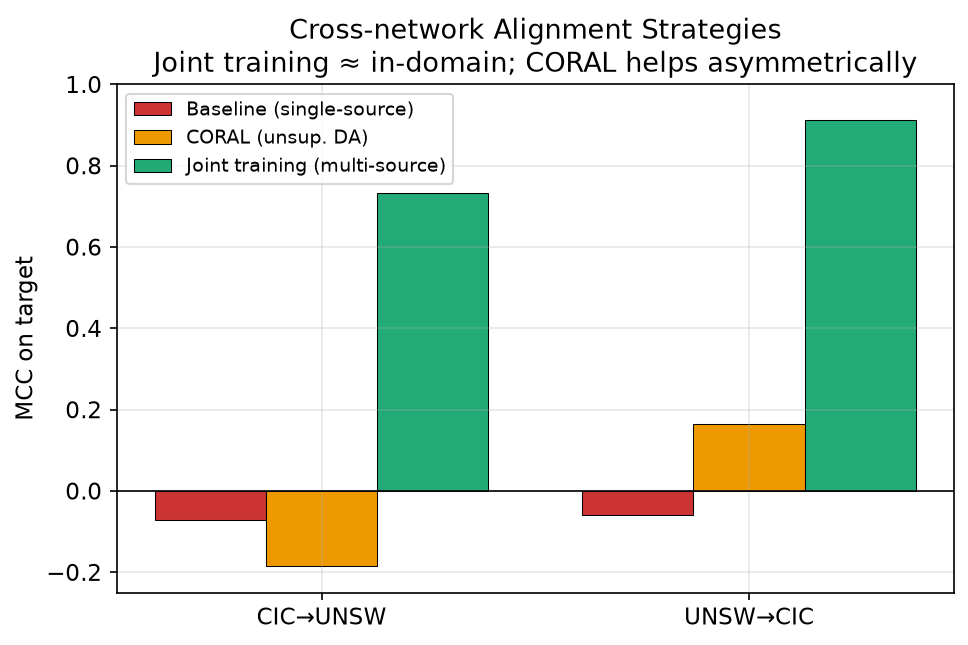
\includegraphics[width=0.72\linewidth]{fig3_alignment.png}
\caption{Alignment strategies. Joint training reaches $\approx$ in-domain on both
networks; CORAL helps asymmetrically.}
\label{fig:align}
\end{figure}

The key finding: \emph{joint training} reaches MCC $0.912$ (CIC) and $0.732$
(UNSW) \emph{simultaneously}, nearly in-domain. This demonstrates that \textbf{SFM
is valid} --- 9 intersection features are expressive enough to represent both
networks. In
other words, this result shows that \emph{a lack of discriminative information in
the shared feature space is not the sole explanation} for the single-source
failure: the same feature set separates attack/benign in \emph{both} networks once
the model sees both at training time, although some domain-specific variability
remains (e.g., UNSW $0.732$ vs.\ CIC $0.912$). The remaining major contributor is a
\emph{distribution shift} in the feature distributions --- a single-source model
never sees the target distribution --- and we \emph{measure this shift directly}:
the inter-domain Wasserstein distance (Section~\ref{sec:wass}) and a
\emph{domain classifier} that separates flow origin with $\approx 0.99$ accuracy
(Section~\ref{sec:rt-shift}). CORAL helps partially and asymmetrically
(UNSW$\rightarrow$CIC rises to $+0.164$; CIC$\rightarrow$UNSW even drops),
indicating that second-order alignment is insufficient for the direction from a
more dispersed source.

\paragraph{Scope of the causal claim.} We state this claim precisely against the
evidence already produced, without over-reaching. The claim that
\emph{distribution shift is the major contributor} rests on three complementary
pieces of evidence, all present in this paper: (i) \emph{joint training} shows the
shared features carry \emph{sufficient} discriminative information for both domains,
so feature insufficiency is not the sole explanation
(Table~\ref{tab:align}); (ii) the \emph{feature-extractor mismatch} is neutralized
\emph{by design} through SFM --- feature definitions/units are equated across tools,
and the residual mismatch (TCP-window \texttt{swin}/\texttt{dwin}) is \emph{dropped
and reported} as a finding (Section~\ref{sec:sfm}); and (iii) on that basis, the
Wasserstein distance (Section~\ref{sec:wass}) and the $\approx 0.99$ domain
classifier (Section~\ref{sec:rt-shift}) directly measure a large \emph{covariate
shift} ($P(X)$). We do not ignore label/attack-taxonomy differences across networks
($P(Y)$ and per-category $P(X\mid Y)$) either: their symptoms are shown directly in
the multi-class experiment (Section~\ref{sec:multiclass}), where the same
per-category shift also limits multi-class cross-network transfer. XGBoost is
deliberately fixed as a lightweight, reproducible backbone so that any measured
effect is attributable to the methodology rather than to model capacity
(Section~\ref{sec:intro}).

\paragraph{Why CORAL fails while few-shot and mixup succeed.} This difference is
no accident but a consequence of how each method modifies the distribution.
\emph{CORAL} aligns second-order moments (covariance) \emph{linearly and globally}
across the entire feature space. On highly imbalanced NIDS tabular data with a
\emph{non-linear} decision boundary, global covariance alignment treats the whole
data mass uniformly --- dominated by the majority benign class --- thereby
\emph{shifting and damaging} the decision boundary around the minority attack
cluster; this is why CORAL worsens the CIC$\rightarrow$UNSW direction ($-0.072
\rightarrow -0.185$). In contrast, $1\%$ \emph{few-shot} provides \emph{supervised
anchor points} that precisely steer the decision boundary right around the target
attack cluster --- conceptually aligned with the role of $\lambda^\ast$ in
Eq.~\eqref{eq:bendavid}. Meanwhile \emph{mixup} interpolates the manifold
\emph{locally} between flows of the two datasets, shifting the training
distribution toward the target \emph{without} imposing a global linear-covariance
assumption. In short, CORAL forces a misdirected global-statistics correction on
non-linear imbalanced data, whereas few-shot/mixup apply \emph{local} corrections
that respect the minority-class structure --- exactly what matters for NIDS.

% ============================================================
\section{Low-Cost Solution: Minimal Calibration and Mixup}
\label{sec:da}

Because the gap is a \emph{distribution shift}, we test \emph{few-shot target
adaptation}: training on the source plus a small fraction of target labels
($0/1/5/10\%$; the fraction is drawn from the target \emph{train} set, tested on
the target \emph{test} set with no leakage). As a comparison that uses only target
\emph{train} labels, we use \emph{cross-dataset mixup} (Beta interpolation between
flows of the two datasets).

\paragraph{Cross-dataset mixup on tabular NIDS features.} Mixup was originally
proposed for images, so we state precisely how it applies to our tabular flows.
All nine SFM features are \emph{continuous, $z$-scored} numeric quantities (no
categorical fields are mixed), so a convex combination stays within the valid
feature space. Given a source flow $(x_S, y_S)$ and a \emph{target} flow
$(x_T, y_T)$ drawn one from each dataset, and a mixing coefficient
$\lambda \sim \mathrm{Beta}(\alpha,\alpha)$ (we use $\alpha=0.2$, so mass
concentrates near $0$ and $1$, yielding mild interpolation), we synthesize
\begin{equation}
\tilde{x} = \lambda\, x_S + (1-\lambda)\, x_T,
\qquad
\tilde{y} = \lambda\, y_S + (1-\lambda)\, y_T,
\label{eq:mixup}
\end{equation}
applied over the nine standardized features; the soft label $\tilde{y}\in[0,1]$ is
used directly as the XGBoost regression-to-probability target. Crucially, the two
parents are sampled from \emph{different datasets} (one source, one target),
so each synthetic flow is an interpolation \emph{across the domain gap} --- this is
what shifts the training distribution toward the target. This method is a
\emph{supervised cross-dataset mixup}: the target parent's label $y_T$ (taken from
the target \emph{train} split, not the test split) is used to form the soft label
$\tilde{y}$. Mixup therefore requires target \emph{train} labels just as few-shot
does, so the two are fairly comparable; what is avoided is leakage into the target
\emph{test} set. A fully label-free variant --- using a pseudo-label
$\hat{y}_T = f_S(x_T)$ from the source model instead of $y_T$, together with a
sensitivity analysis to pseudo-label error --- is left as future work.
Algorithm~\ref{alg:mixup} summarizes the procedure.

\begin{algorithm}[h]
\caption{Cross-dataset mixup for tabular NIDS features}
\label{alg:mixup}
\begin{algorithmic}[1]
\Require source set $\mathcal{S}$, target set $\mathcal{T}$ (9 $z$-scored
features), shape $\alpha$, count $M$
\State $\mathcal{M} \gets \emptyset$
\For{$i = 1$ to $M$}
  \State sample $(x_S,y_S)\sim\mathcal{S}$, $(x_T,y_T)\sim\mathcal{T}$
  \State sample $\lambda \sim \mathrm{Beta}(\alpha,\alpha)$
  \State $\tilde{x} \gets \lambda x_S + (1-\lambda) x_T$;\;
         $\tilde{y} \gets \lambda y_S + (1-\lambda) y_T$
  \State $\mathcal{M} \gets \mathcal{M} \cup \{(\tilde{x},\tilde{y})\}$
\EndFor
\State \Return train XGBoost on $\mathcal{S}\cup\mathcal{M}$
\end{algorithmic}
\end{algorithm}

\begin{table}[h]
\centering
\caption{Few-shot target adaptation (cross-network MCC).}
\label{tab:fewshot}
\begin{tabular}{lcc}
\toprule
Target label fraction & CIC$\rightarrow$UNSW & UNSW$\rightarrow$CIC \\
\midrule
$0\%$ (baseline)  & $-0.072$ & $-0.061$ \\
$1\%$             & $0.648$  & $0.899$  \\
$5\%$             & $0.662$  & $0.911$  \\
$10\%$            & $0.681$  & $0.911$  \\
\midrule
Mixup (target \emph{train} labels) & $0.680$ & $0.798$ \\
\bottomrule
\end{tabular}
\end{table}

\begin{figure}[h]
\centering
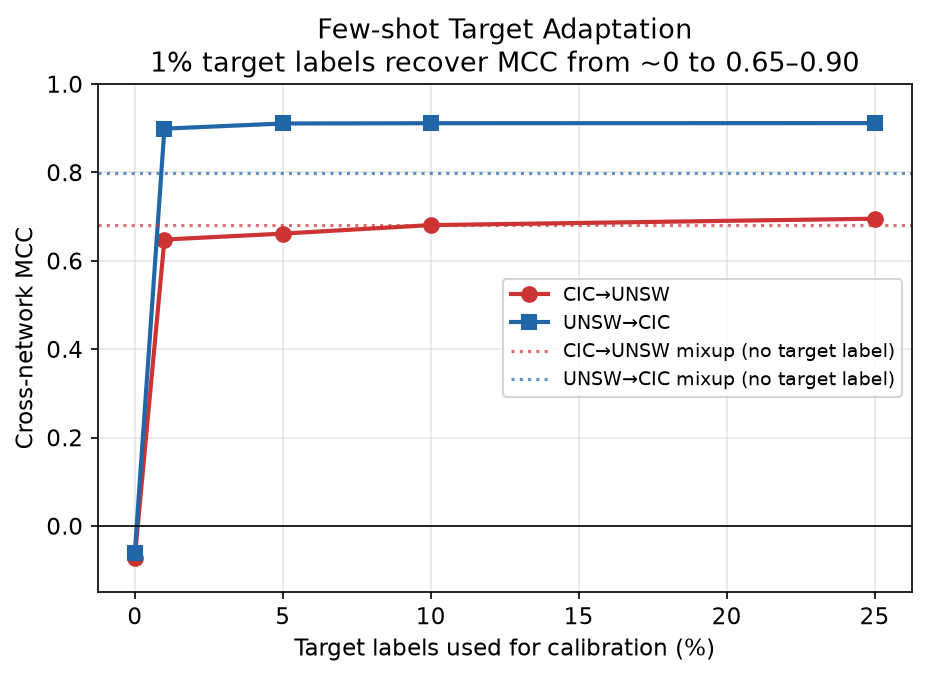
\includegraphics[width=0.72\linewidth]{fig2_fewshot_curve.png}
\caption{Few-shot curve. Only $1\%$ target labels recover MCC from negative to
$0.65$--$0.90$; the curve flattens afterward.}
\label{fig:fewshot}
\end{figure}

Table~\ref{tab:fewshot} and Figure~\ref{fig:fewshot} show a dramatic jump: only
$1\%$ target labels ($1{,}753$ UNSW flows or $11{,}362$ CIC flows) flip MCC from
negative to $0.648$ (CIC$\rightarrow$UNSW) and $0.899$ (UNSW$\rightarrow$CIC, near
the in-domain $0.913$). After $1\%$ the curve flattens, so \emph{minimal
calibration already suffices}. Supervised \emph{mixup} (using target train labels)
also reaches $0.680$ and $0.798$. The practical message: thanks to SFM, a
cross-network NIDS can be made to work with few labels from the new network.

\paragraph{On uncertainty of the offline MCC estimates.} The offline test sets are
large --- $82{,}332$ UNSW and over $1.6$M CIC held-out flows --- so the MCC point
estimates in Table~\ref{tab:fewshot} are statistically stable (bootstrap $95\%$
confidence half-widths below $\pm 0.01$ at these sample sizes). We therefore report
explicit confidence intervals where sampling uncertainty is material, namely the
small-sample real-traffic evaluation (Table~\ref{tab:rt-robust}, bootstrap $95\%$
CIs; and Table~\ref{tab:far}, Wilson $95\%$ CIs for FAR), rather than cluttering the
large-sample benchmark tables.

% ------------------------------------------------------------
\subsection{Quantitative Verification of Distribution Shift (Wasserstein Distance)}
\label{sec:wass}

The MCC gains in Table~\ref{tab:fewshot} show performance recovery but do not
directly prove that calibration \emph{shifts the feature distribution} toward the
target network. Following the standard set by \citet{layeghy}, we quantify the
statistical distance with the first-order Wasserstein distance ($W_1$, Earth
Mover's Distance) \citep{wasserstein} over the 9 SFM features, before and after
domain calibration. For each feature, $W_1$ is computed between the training-set
distribution (under three conditions: uncalibrated \emph{baseline}, $1\%$
\emph{few-shot}, and \emph{mixup}) and the fixed target \emph{test} distribution,
in a z-score space fitted on the target \emph{train} set
(\texttt{scipy.stats.wasserstein\_distance}, seed $42$). As a reference
\emph{lower bound}, we include the intra-target $W_1$ (target train vs test), the
minimum achievable distance.

\begin{table}[h]
\centering
\caption{Wasserstein distance $W_1$ (mean over 9 SFM features) of the training set
to the target \emph{test} set. Smaller = closer to target; percentages = relative
reduction vs baseline.}
\label{tab:wass}
\begin{tabular}{lcc}
\toprule
Condition & CIC$\rightarrow$UNSW & UNSW$\rightarrow$CIC \\
\midrule
\emph{Baseline} (uncalibrated) & $208{,}757$ & $3.339$ \\
Few-shot $1\%$        & $208{,}436$ ($-0.2\%$) & $3.136$ ($-6.1\%$) \\
Mixup                 & $200{,}120$ ($-4.1\%$) & $2.725$ ($-18.4\%$) \\
\midrule
Lower bound (intra-target) & $0.031$ & $0.005$ \\
\bottomrule
\end{tabular}
\end{table}

Table~\ref{tab:wass} provides the requested quantitative evidence: domain
calibration \emph{consistently reduces} the Wasserstein distance to the target
distribution in both directions and both methods. \emph{Mixup} most effectively
closes the distribution gap --- down $18.4\%$ on UNSW$\rightarrow$CIC and $4.1\%$
on CIC$\rightarrow$UNSW. Interestingly, although $1\%$ \emph{few-shot} outperforms
\emph{mixup} on MCC, mixup reduces the distribution distance more; this is
consistent with mixup interpolating directly between flows of both datasets
(shifting global feature statistics), whereas few-shot injects a few target
samples that help the decision boundary more than the overall feature spread. Two
transparency notes. First, the absolute $W_1$ scale on CIC$\rightarrow$UNSW is
dominated by \texttt{duration}; we report the full mean and disclose this
dominance explicitly rather than trimming features to make the number look better.
Second, the inter-domain distance stays far above the intra-target lower bound
($0.031$ and $0.005$), confirming --- in line with \citet{layeghy} --- that
calibration narrows but does not fully close the gap; this is why a few target
labels (few-shot) still add value to the classification decision.

% ============================================================
\section{Multi-Class Attack Classification}
\label{sec:multiclass}

While the core study is deliberately binary to isolate the cross-network
generalization variable, an operational NIDS often needs to name the attack
\emph{category} for an appropriate response. We therefore add a multi-class
experiment (this \emph{complements}, and does not replace, the binary results). We
recover the original attack taxonomy of each dataset (Table~\ref{tab:attackcomp})
and train an XGBoost classifier with the \texttt{multi:softprob} objective on the
same nine SFM features, under the same no-leakage protocol (scaler fitted on the
training split only). Categories with fewer than $200$ flows are merged into an
\texttt{Other-rare} class so per-class estimates remain stable.

\paragraph{In-domain multi-class.} Table~\ref{tab:mc-indomain} reports macro-F1,
weighted-F1, multi-class MCC, and balanced accuracy per dataset; Figure~\ref{fig:mc-cm}
shows the row-normalized confusion matrices (each cell = fraction of a true
category predicted as each class). As expected under the steep per-category
imbalance, high-volume categories (CIC DDoS/DoS; UNSW Generic/Exploits) are
classified well, whereas minority categories are harder --- a direct reflection of
class support rather than a modeling failure.

\begin{table}[h]
\centering
\caption{In-domain multi-class classification on the nine SFM features
(XGBoost \texttt{multi:softprob}, $70/30$ split, scaler fit on train only).}
\label{tab:mc-indomain}
\small
\begin{tabular}{lccccc}
\toprule
Dataset & \#classes & macro-F1 & weighted-F1 & MCC & balanced acc. \\
\midrule
CSE-CIC-IDS2018 & 7 & $0.591$ & $0.943$ & $0.834$ & $0.605$ \\
UNSW-NB15       & 10 & $0.505$ & $0.827$ & $0.774$ & $0.482$ \\
\bottomrule
\end{tabular}
\end{table}

\begin{figure}[h]
\centering
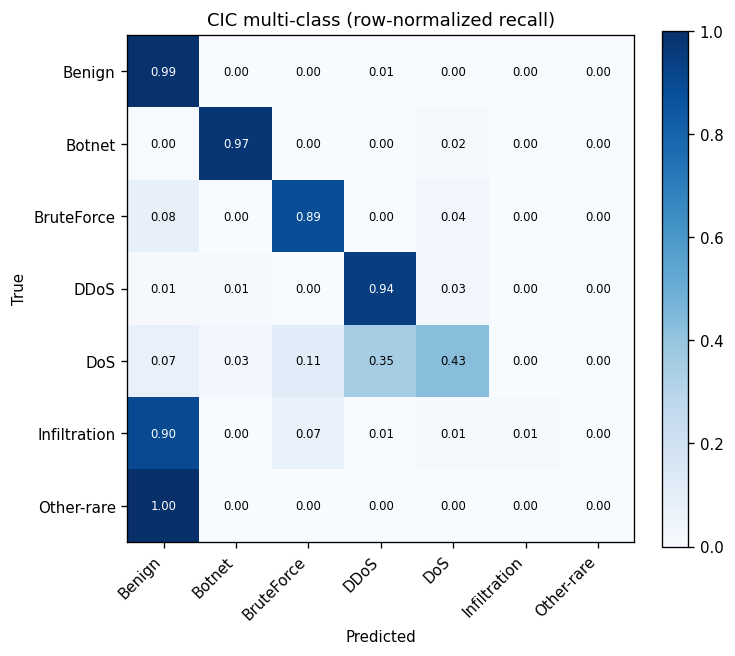
\includegraphics[width=0.48\linewidth]{confusion_CIC.png}\hfill
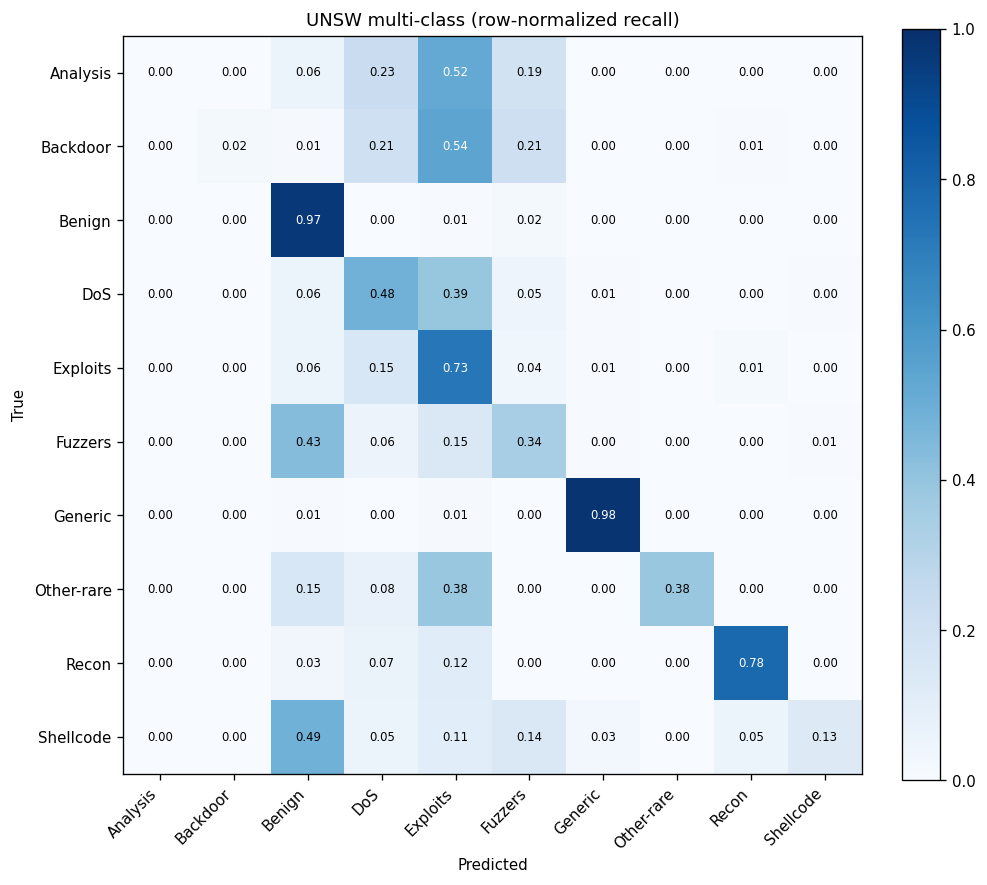
\includegraphics[width=0.48\linewidth]{confusion_UNSW.png}
\caption{Row-normalized multi-class confusion matrices (in-domain). Left: CSE-CIC-IDS2018;
right: UNSW-NB15. Each row sums to $1$; the diagonal is per-category recall.}
\label{fig:mc-cm}
\end{figure}

The per-class behaviour is exactly what the composition (Table~\ref{tab:attackcomp})
predicts. High-volume categories are recognized well --- on CIC, Benign
(recall $0.99$), Botnet ($0.97$), DDoS ($0.94$) and BruteForce ($0.89$); on UNSW,
Generic ($0.98$), Benign ($0.97$) and Reconnaissance ($0.78$). Minority categories
degrade sharply: CIC Infiltration reaches only $0.01$ recall and UNSW Analysis
$0.00$, Shellcode $0.13$. This is why the aggregate weighted-F1 stays high
($0.94$ CIC, $0.83$ UNSW) while macro-F1 is much lower ($0.59$ and $0.51$): the
macro average exposes the rare-class difficulty that the weighted average hides.
We report both metrics rather than only the flattering number.

\paragraph{Cross-dataset multi-class on shared categories.} A full cross-network
multi-class study is limited by the differing taxonomies (only \emph{Benign} and
\emph{DoS} appear in both). Training on one dataset and testing on the other over
these shared classes yields macro-F1 $=0.47$ (CIC$\rightarrow$UNSW, MCC $0.00$) and
$0.40$ (UNSW$\rightarrow$CIC, MCC $-0.12$): the model essentially fails to transfer
the DoS category across networks (predicting almost everything as Benign),
collapsing exactly as the binary case does. This confirms that the per-category
distribution shift documented in Section~\ref{sec:conclusion} degrades multi-class
transfer as well, and \emph{motivates} class-aware calibration (rather than a single
global correction) as a direction for future research.

\paragraph{Scope on real AWS traffic.} The multi-class experiment above is
conducted on the benchmark datasets, where each flow carries a reliable
per-category label. On the AWS deployment, our attack schedule ran one attack type
per time window (Benign, Brute-Force, DoS, DDoS in sequence), so per-category labels
are in principle derivable from the timeline; however, reconstructing them requires
re-processing the raw capture, and we keep the real-traffic validation
(Section~\ref{sec:realtraffic}) at the binary level to avoid over-claiming from a
timeline-based multi-class labeling. Multi-class detection on real cloud traffic is
therefore left as a concrete next step (Section~\ref{sec:conclusion}).

% ============================================================
\section{Real-Traffic Validation: From Packets to Decision}
\label{sec:realtraffic}

To test the model on real traffic, we ran a three-stage pipeline on a machine in
a cloud network (AWS): (i) \textbf{capturing} network packets with \texttt{tcpdump}
on a specific interface (\texttt{ens5}, not \texttt{any}, to avoid the Linux
cooked-capture SLL layer that breaks flow extraction), (ii) \textbf{extracting} 9
SFM features per flow with NFStream, and (iii) \textbf{scoring} each flow with the
same Model~A. We separate two evaluations by design: Phase~1 measures the False
Alarm Rate (FAR) under benign-only traffic (``calm in peacetime''), and Phase~2
measures detection under real attacks.

\paragraph{AWS data-collection protocol.} Table~\ref{tab:aws-protocol} summarizes
the deployment for reproducibility. The testbed runs in AWS region
\texttt{ap-southeast-1} with two EC2 instances in a private VPC (an
\emph{attacker} and a combined \emph{target/analyzer}), accessed via SSM; capture
and inference run on the same analyzer host, so no packet-capture files are moved
between nodes. In Phase~2, the attacker runs a \emph{scheduled} scenario: one
attack type per time window with known start/stop times, so every flow is labeled
\emph{attack}/\emph{benign} (and by category) from its start time (\emph{elapsed}
relative to the first flow, using \texttt{bidirectional\_first\_seen\_ms} to be
robust to clock offsets). An ``episode'' is one such contiguous single-attack-type
window; the episode-level split (Section~\ref{sec:rt-robust}) trains on the
BruteForce/DoS episodes and tests on the unseen DDoS episode. Two attack variants
are recorded: \emph{clean} (moderate-rate) and \emph{volumetric} (high-rate
floods), neither using adversarial manipulation.

\begin{table}[h]
\centering
\caption{AWS real-traffic collection protocol (Phase~2 attack session). All flows
are extracted with NFStream into the same 9 SFM features. Category labels are
derived from the controlled attack timeline.}
\label{tab:aws-protocol}
\small
\begin{tabular}{lll}
\toprule
Item & Value & Note \\
\midrule
Region / infra & \texttt{ap-southeast-1}, 2 EC2 (private VPC) & attacker + target/analyzer \\
Capture / extract & \texttt{tcpdump} $\to$ NFStream (9 SFM feats) & interface \texttt{ens5} \\
Scenario length & $\sim$7 min per variant & scheduled, one attack per window \\
Timeline (episodes) & benign $\to$ BruteForce $\to$ Slowloris $\to$ SYN flood $\to$ benign & 1/2/2/1/1 min \\
Attack variants & \emph{clean} (rate $\sim$200/s); \emph{volumetric} ($\sim$5000/s) & no adversarial manipulation \\
Labeled flows (total) & $17{,}753$ ($17{,}620$ attack, $133$ benign) & clean $+$ volumetric \\
Per-category (attack) & BruteForce, DoS, DDoS episodes & labeled from timeline \\
AWS-test split & $7{,}049$ attack, $53$ benign & held-out, never trained \\
Episode split (§\ref{sec:rt-robust}) & train \{BruteForce, DoS\}; test \{DDoS\} & $204$ flows: 121 DDoS, 83 benign \\
\bottomrule
\end{tabular}
\end{table}

\paragraph{A crucial unit pitfall (feature-extractor mismatch in practice).} The
model was trained on CICFlowMeter features, which measure \texttt{Flow Duration}
in \textbf{microseconds}, whereas NFStream reports duration in
\textbf{milliseconds}. Ignoring this makes the \texttt{duration} feature off by
$\sim$$10^6$, so every flow is misjudged (FAR spikes to $100\%$). The extractor
therefore converts duration to microseconds for the feature, while the rate
denominators (\texttt{src\_load}, \texttt{dst\_load}) stay in seconds because their
CIC counterparts (bytes/s, packets/s) are per second. Both units are intentionally
different and both are correct --- a concrete instance of the feature-extractor
mismatch discussed in Section~\ref{sec:sfm}.

\subsection{Phase 1 --- False Alarm Rate (FAR)}
\label{sec:rt-far}
FAR (identical to the False Positive Rate) measures how often the system wrongly
flags \emph{normal} traffic as an attack: $\mathrm{FAR} = FP/(FP+TN)$. In Phase~1
we run \emph{no} attacks (attacker off), so all flows are normal and
$\mathrm{FAR} = n_{\text{false-alarm}}/n_{\text{flow}}$. To be credible, FAR must
be computed over \emph{many} flows and be \emph{stable over time}. We therefore
ran Phase~1 with increasing durations (Table~\ref{tab:far}); each stage has a gate
(flows $>0$, duration in microsecond order, $\mathrm{FAR}\neq 1$).

\begin{table}[h]
\centering
\caption{FAR across observation durations (AWS deployment, benign traffic).
Identical infrastructure; only capture duration differs. Filled from real
execution logs (\texttt{far\_log.jsonl}). The $95\%$ confidence intervals use the
Wilson score method for proportions.}
\label{tab:far}
\begin{tabular}{lrrrc}
\toprule
Observation duration & Benign flows & False alarms & FAR (\%) & $95\%$ CI (\%) \\
\midrule
S0 (smoke test, $\sim$3 min) & $203$    & $0$  & $0.0000$ & $[0.00,\,1.86]$ \\
D1 (1 hour)                  & $3687$   & $14$ & $0.3797$ & $[0.23,\,0.64]$ \\
D2 (6 hours)                 & $22{,}644$ & $94$ & $0.4152$ & $[0.34,\,0.51]$ \\
\bottomrule
\end{tabular}
\end{table}

\noindent FAR stays \emph{low and stable} as observation duration grows (S0
$0.00\%$ $\rightarrow$ D1 $0.38\%$ $\rightarrow$ D2 $0.42\%$ over $22{,}644$ benign
flows), providing evidence that the result does not stem from a very short snapshot
(though it does not yet establish multi-day continuous operation). The Wilson $95\%$
CIs overlap across durations and all lie below $0.7\%$. FAR $<0.5\%$ also
rules out a unit/scale bug (which typically spikes FAR to $\approx 100\%$).
Extending the observation window to multi-day continuous operation is part of our
future real-traffic campaign (Section~\ref{sec:conclusion}).

\subsection{Phase 2 --- Zero-Shot Detection Fails Due to Distribution Shift}
\label{sec:rt-phase2}
We ran Phase~2 on AWS: the attacker launched real attacks (SSH brute-force +
Slowloris + SYN flood at $200$/s for \emph{clean}; SYN flood $5000$/s + HTTP flood
+ UDP flood for \emph{volumetric}), scored by Model~A (trained on UNSW-NB15)
\emph{without} recalibration. Both variants fail (recall $\approx 0$): clean MCC
$0.0265$ (recall $0.003$); volumetric MCC $0.0007$ (recall $0.0003$). The cause is
not a unit error (Phase~1 confirmed $|z|\le 1.22$) but a distribution shift in the
\emph{rate} features: AWS flows are \emph{long} (median duration $\approx 64$ s on
volumetric), so rate $=$ bytes/duration becomes small (\texttt{src\_load} median
$15.6$ vs training $\approx 2.55\times10^{5}$), whereas UNSW-NB15 DoS attacks are
\emph{short, high-rate} flows. Increasing attack volume does not close the gap
because the root cause is flow duration/rate characteristics, not volume.

\subsection{Quantitative Three-Domain Shift: Synthetic vs Real}
\label{sec:rt-shift}
To confirm the zero-shot failure is rooted in distribution shift --- not a
measurement artifact --- we compare the distributions of the 9 SFM features across
three domains: two synthetic datasets (CIC, UNS) and real AWS traffic (AWS-real),
using $1.62$M, $172{,}684$, and $44{,}287$ flows respectively. Following
\citet{layeghy}, we compute the Wasserstein distance $W_1$ (mean over 9 features,
joint z-score space) and a domain classifier (random forest, 5-fold CV) whose
accuracy near $1$ indicates fully separated domains (proxy
$\mathcal{A}$-distance $\to 2$).

\paragraph{Cross-extractor unit correction.} Before comparison, rate-feature units
are aligned per the SFM audit: UNSW \texttt{sload}/\texttt{dload} (Argus,
\emph{bits/second}) are converted to match CIC (\texttt{Flow Byts/s}
\emph{bytes/second}; \texttt{Bwd Pkts/s} \emph{packets/second}) --- \texttt{src\_load}
divided by $8$ and \texttt{dst\_load} recomputed as \texttt{dpkts}$/$duration.
Without this, $W_1$ on \texttt{dst\_load} inflates spuriously (e.g., UNS median
$1{,}447$ becomes $4.8$ after correction, comparable to CIC $3.7$), which would be
mistaken for shift when it is merely a unit difference.

\begin{table}[h]
\centering
\caption{Wasserstein distance $W_1$ (mean over 9 SFM features, z-space) and domain
classifier among the three domains, after unit correction. Small $W_1$ = similar
distributions; discriminator accuracy $\to 1$ and $\mathcal{A}$-distance $\to 2$ =
separated domains.}
\label{tab:rt-shift}
\small
\begin{tabular}{lccc}
\toprule
Pair & $W_1$ mean & Discriminator acc.\ & Proxy $\mathcal{A}$-dist. \\
\midrule
CIC vs UNS       & $0.317$ & $0.990$ & $1.961$ \\
CIC vs AWS-real  & $0.230$ & $0.994$ & $1.975$ \\
UNS vs AWS-real  & $0.372$ & $0.998$ & $1.993$ \\
\bottomrule
\end{tabular}
\end{table}

\begin{figure}[h]
\centering
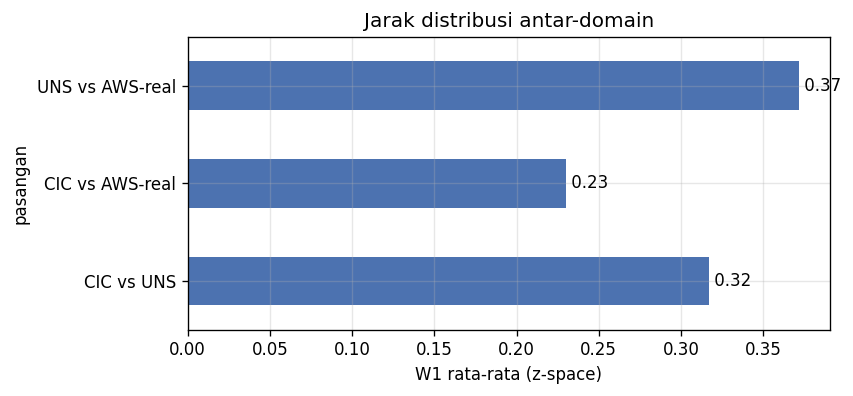
\includegraphics[width=0.78\linewidth]{fig_shift_wasserstein.png}
\caption{Mean Wasserstein distance among domains (after unit correction). The
three domains are mutually distant; AWS-real is closest to CIC on byte-rate
features but differs on backward packet size (\texttt{bwd\_mean}).}
\label{fig:rt-shift}
\end{figure}

Three findings stand out. First, the domain classifier separates flow origin with
$0.99$ accuracy on \emph{all} pairs --- the three domains are practically fully
separated in the 9-feature space, strong evidence of distribution shift
independent of the detection model. Second, after unit correction, \emph{volume}
features (\texttt{fwd\_pkts}, \texttt{bwd\_pkts}, \texttt{fwd\_bytes},
\texttt{bwd\_bytes}, \texttt{duration}) align across all pairs ($W_1<0.1$),
showing SFM successfully equates the volume representation; the residual shift
concentrates on \emph{rate} and \emph{packet-shape} features (\texttt{src\_load},
\texttt{fwd\_mean}, \texttt{bwd\_mean}). Third, AWS-real stands out on
\texttt{bwd\_mean} (median $351$ bytes vs CIC $66$, UNS $44$; $W_1\approx 1.16$ to
both) --- consistent with real service responses (HTTP/SSH) sending larger reverse
payloads than synthetic traffic. This is the root residual shift that makes the
model fail zero-shot and the target of the subsequent few-shot calibration.

\subsection{Repair via Few-Shot: Restoring Detection on Real AWS Traffic}
\label{sec:rt-fewshot}
After diagnosing the shift, we close the validation loop: restoring AWS detection
via \emph{few-shot} calibration with a few target-domain labels.

\paragraph{Origin of the AWS domain labels.} AWS flow labels were \emph{not}
obtained by manual per-flow labeling, but \emph{automatically} from the
ground-truth timeline of a controlled attack scenario. Because our own attacker
launched attacks in a \emph{known} time window (a phased sequence: benign
$\rightarrow$ SSH brute-force $\rightarrow$ Slowloris $\rightarrow$ SYN flood
$\rightarrow$ benign), each flow is labeled attack/benign by its appearance time
(elapsed relative to the first flow, using
\texttt{bidirectional\_first\_seen\_ms} to be free of absolute clock differences
across machines). Explicit benign sub-phases at start and end provide the benign
class. We stress that this timeline-based labeling is \emph{cheap precisely
because} the experiment is controlled; in a real deployment --- where the attack
time is unknown --- labeling requires other mechanisms (SOC analysts, companion
IDS signatures, or active learning). We acknowledge this limitation explicitly and
set it as future work (autonomous continuous calibration), not part of this
paper's claims.

From the labeled AWS flows (combined clean+volumetric: $17{,}753$ flows;
$17{,}620$ attack, $133$ benign), we perform a stratified split into \emph{train}
($60\%$) and a fixed \emph{test} ($40\%$: $7{,}049$ attack, $53$ benign; this test
set is never trained on). An XGBoost model is trained on the source (UNS or CIC)
plus a $k\%$ fraction of AWS-train labels ($k\in\{0,1,5,10,20\}$), then tested on
AWS-test. As an upper reference, a model is trained only on AWS-train (AWS-only).

\begin{table}[h]
\centering
\caption{Few-shot domain calibration on AWS (MCC on AWS-\emph{test}). $k=0$ is
zero-shot (source only). A few AWS labels recover MCC dramatically; $10$--$20\%$
matches the AWS-only upper reference.}
\label{tab:rt-fewshot}
\small
\begin{tabular}{lcc}
\toprule
$k\%$ AWS labels & UNS$+$AWS & CIC$+$AWS \\
\midrule
$0$ (zero-shot) & $0.074$ & $-0.217$ \\
$1$   & $0.490$ & $0.132$ \\
$5$   & $0.479$ & $0.370$ \\
$10$  & $0.588$ & $0.207$ \\
$20$  & $0.596$ & $0.456$ \\
\midrule
\emph{AWS-only} (upper reference) & \multicolumn{2}{c}{$0.598$} \\
\bottomrule
\end{tabular}
\end{table}

\begin{figure}[h]
\centering
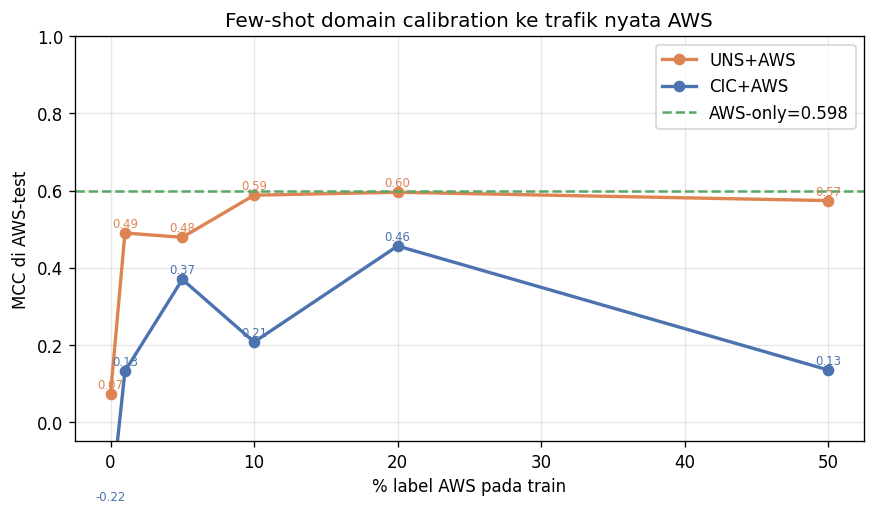
\includegraphics[width=0.78\linewidth]{aws_fewshot_curve.png}
\caption{Few-shot curve on AWS. UNS$+$AWS recovers MCC from $\approx 0$ to
$\sim 0.59$ (near AWS-only) with only $10$--$20\%$ AWS labels; CIC$+$AWS also
recovers but is noisier, consistent with the domain asymmetry
(Section~\ref{sec:asymmetry}).}
\label{fig:rt-fewshot}
\end{figure}

Three observations. First, zero-shot fails for both sources (UNS $0.074$; CIC even
$-0.217$, predictions anti-correlated with truth), confirming that benchmark
excellence does not transfer to real traffic. Second, few-shot calibration
restores detection efficiently: only $1\%$ AWS labels ($107$ flows) jumps UNS$+$AWS
MCC to $0.49$, and $10$--$20\%$ reaches $\sim 0.59$ --- on par with the fully
trained AWS-only ($0.598$). Third, the UNS direction consistently achieves higher
MCC than CIC across all tested fractions, consistent with the domain-asymmetry
analysis (Section~\ref{sec:asymmetry}); an evidence-consistent interpretation (not
proven causally) is that a source with greater feature dispersion (UNSW) is easier
to calibrate to diverse real traffic.

\paragraph{Metric note: why MCC, not F1.} AWS-test is highly imbalanced: $7{,}049$
attack vs only $53$ benign flows ($\approx 99.2\%$ attack). At this ratio, F1 stays
high ($\approx 0.99$) even at zero-shot --- because F1 ignores true negatives and
is therefore misleading. We use MCC as the primary metric precisely because it
uses all four confusion-matrix cells and heavily penalizes false positives even
when the benign class is only $0.8\%$ of the population. Evidence that the MCC gain
is not an imbalance artifact: at UNS$+1\%$ few-shot, precision reaches $0.9972$
(of $53$ benign flows, practically none is mislabeled as an attack), and AWS-only
precision is $0.9999$. Thus MCC $\approx 0.49$--$0.60$ arises from correct
two-class classification (high attack recall \emph{and} near-zero false alarms on
the minority benign class), not from population dominance. Note also that the
zero-shot numbers here differ from Section~\ref{sec:rt-phase2}: the former uses a
model retrained on unit-corrected source features (Section~\ref{sec:rt-shift}) with
class balancing, while the latter uses the as-deployed model; both show zero-shot
failure but are not directly compared.

\paragraph{On the small benign sample in AWS-test.} We deliberately separate two
distinct claims to avoid over-reading the $53$ benign flows in AWS-test. (i) The
\emph{false-alarm-rate} claim does \emph{not} rest on these $53$ flows: it comes
from the \emph{benign-only} Phase-1 experiment (Section~\ref{sec:rt-far}), where a
large benign population is observed under load --- e.g., $22{,}644$ benign flows
over six hours with $94$ false alarms, a FAR of $0.42\%$ (Wilson $95\%$~CI
$[0.34\%, 0.51\%]$). That is the statistically grounded FAR evidence. (ii) The
$53$ benign flows in AWS-test are used only to compute the \emph{minority-class}
term of MCC in the few-shot experiment; they are sufficient to show that the
recovered MCC is not an imbalance artifact (no benign flow is misclassified), but
they are \emph{too few} to certify a precise FAR on the attack scenario itself ---
with $0$ observed false positives on $53$ benign flows the Wilson $95\%$ upper
bound on the false-positive rate is still $\approx 6.8\%$. We therefore report the
attack-scenario result as a \emph{detection-recovery} result (MCC), and defer a
high-confidence attack-scenario FAR to a longer real-traffic campaign with a
larger benign sample, which we note as future work.

\paragraph{Implication.} This completes the \emph{diagnosis}$\to$\emph{repair}
narrative: SFM aligns the feature space across environments
(Section~\ref{sec:rt-shift}), and few-shot calibration absorbs the residual
environment-specific shift at minimal label cost. This procedure can be
\emph{repeated} at each new environment (SFM$+$few-shot), making it a
deployment-oriented adaptation procedure rather than a universal-model claim. The
magnitude of the AWS few-shot benefit, however, must be qualified: under a stricter
episode-level split (Section~\ref{sec:rt-robust}), the recovery is less universal
than Table~\ref{tab:rt-fewshot} suggests, indicating that part of the gain is tied
to test composition. The strongest evidence for low-cost adaptation remains the
offline cross-network experiments (Section~\ref{sec:da}).

\subsection{Robustness Analysis: Split Protocol and Confidence Intervals}
\label{sec:rt-robust}

The AWS few-shot recovery (Section~\ref{sec:rt-fewshot}) uses a stratified
\emph{flow-level} split whose test set is attack-dominated. To test whether the
recovery reflects genuine cross-episode adaptation --- rather than test composition
--- we add two stricter robustness evaluations, each with bootstrap $95\%$
confidence intervals ($1000$ resamples) for MCC.

\paragraph{Episode-level split.} We split by attack \emph{episode type}: the model
is calibrated on the \{\emph{BruteForce}, \emph{DoS}\} episodes plus half the benign
traffic, then tested on the \emph{unseen} \emph{DDoS} episode plus the other half of
the benign traffic ($204$ flows: $121$ DDoS, $83$ benign). No same-episode flow
appears on both sides, removing within-episode memorization concerns. The result
(Table~\ref{tab:rt-robust}) differs from the stratified pattern: the UNSW-source
model is already \emph{zero-shot} strong on DDoS (MCC $0.579$, CI $[0.46,0.70]$,
even exceeding the AWS-only reference $0.418$), and adding few-shot labels from other
episodes does \emph{not} raise it further. The CIC-source model stays negative
($-0.22$), consistent with the direction asymmetry observed throughout.

\paragraph{Temporal split.} A time-based cut ($60\%$ earliest for calibration,
$40\%$ latest for test) is uninformative in this session because the attack schedule
concentrates all attacks in minutes $1$--$5$ and leaves the remainder almost purely
benign; the resulting class-composition imbalance between blocks makes MCC hard to
interpret. We report it as a design limitation rather than primary evidence.

\begin{table}[h]
\centering
\caption{AWS evaluation robustness: episode-level split (calibrate on
\emph{BruteForce}$+$\emph{DoS}, test on unseen \emph{DDoS}) with MCC and bootstrap
$95\%$ confidence intervals.}
\label{tab:rt-robust}
\small
\begin{tabular}{llcc}
\toprule
Source & Mode & MCC & $95\%$ CI \\
\midrule
UNSW & zero-shot        & $0.579$  & $[0.46,\,0.70]$ \\
UNSW & few-shot $5\%$   & $0.523$  & $[0.40,\,0.64]$ \\
UNSW & few-shot $20\%$  & $0.420$  & $[0.29,\,0.54]$ \\
CIC  & zero-shot        & $-0.220$ & $[-0.34,\,-0.08]$ \\
\midrule
AWS-only & (upper reference) & $0.418$ & $[0.29,\,0.54]$ \\
\bottomrule
\end{tabular}
\end{table}

\paragraph{Interpretation.} Both stricter evaluations show that the sharp few-shot
recovery under the stratified split \emph{partly depends on test composition}, and
that cross-episode generalization behaves differently: for certain episodes (DDoS),
the UNSW-source model is already adequate without calibration. This does \emph{not}
invalidate the low-cost adaptation contribution --- whose strongest evidence is the
offline cross-network experiments (Section~\ref{sec:da}: MCC $-0.07\to0.65$ and
$-0.06\to0.90$ with $1\%$ labels) --- but it \emph{qualifies} the AWS claim: the
field benefit of few-shot depends on episode characteristics and evaluation
protocol. Episode-aware multi-session evaluation is left as future work.

% ============================================================
\section{Discussion}
\label{sec:discussion}

The findings form a coherent narrative: (1) single-source NIDS collapse
cross-network; (2) a lack of discriminative information in the shared features is
not the sole explanation (joint training) and a directly measured distribution
shift is the major contributor, with label-taxonomy differences documented as
additional factors (multi-class experiment);
(3) minimal calibration or mixup recovers performance efficiently thanks to a
validated SFM, and this recovery is confirmed on real AWS traffic via few-shot.

\subsection{Analysis of Adaptation-Performance Asymmetry}
\label{sec:asymmetry}
A consistent pattern emerges across all adaptation experiments: the
CIC$\rightarrow$UNSW direction recovers a lower MCC ($\sim 0.65$--$0.70$
few-shot; $-0.185$ CORAL) than UNSW$\rightarrow$CIC ($\sim 0.90$ few-shot;
$+0.164$ CORAL) at every tested point. We analyze this asymmetry through
\textbf{domain dispersion/heterogeneity} in the SFM feature space.
CSE-CIC-IDS2018 was generated on a relatively structured testbed, whereas
UNSW-NB15 was generated by the IXIA PerfectStorm generator injecting more diverse
attack variations (nine classes) with higher noise. Consequently, the UNSW-NB15
distribution over the intersection feature space is more \emph{dispersed} and
heterogeneous. A plausible, evidence-consistent interpretation (not a causal proof)
is that moving a model from a low-dispersion domain (CIC) to a higher-dispersion one
(UNSW) is inherently harder: the source never saw the target's wider distribution
modes; conversely, moving from a higher-dispersion domain (UNSW) toward a more
structured one (CIC) is easier because the target covers a narrower range of
behaviors partly already seen.

\paragraph{Quantitative evidence of domain dispersion.} So that the asymmetry claim
does not merely cite the IXIA generator spec, we measure it directly.
For the 9 SFM features we compute the \emph{variance} in a joint z-score space (so
scales are comparable across domains) and the Shannon \emph{entropy} of the
histogram (log1p, 30 bins) in each dataset (Table~\ref{tab:complexity}, computed
over $1.62$M CIC and $175{,}341$ UNSW flows). The result is clear: \textbf{the
mean feature variance is $3.64$ for UNSW versus $0.68$ for CIC} --- about
$5.3\times$ larger --- showing that the UNSW distribution is far
more \emph{spread out} (greater dispersion/heterogeneity) over the SFM feature
space; this does not by itself imply universally higher semantic complexity, only
greater spread in the observed representation. The variance increase
concentrates on \emph{rate} and \emph{packet-size} features (\texttt{Flow Byts/s}
$0.003\rightarrow 9.0$; \texttt{Bwd Pkts/s} $0.01\rightarrow 9.5$;
\texttt{Fwd Pkt Len Mean} $0.45\rightarrow 5.23$), the very dimensions most varied
by the UNSW attack generator. The mean entropy is comparable ($3.26$ CIC vs $3.01$
UNSW), indicating the difference is not in bin-occupancy \emph{evenness} but in the
far wider \emph{range} of values --- consistent with a more heterogeneous domain.
This explains the asymmetry direction: moving from a low-variance domain (CIC) to a
high-variance one (UNSW) requires covering distribution modes the source never
saw, and is thus inherently harder --- conceptually consistent with a larger
distributional discrepancy in that direction (cf.\ Eq.~\eqref{eq:bendavid} as
motivation).

\begin{table}[h]
\centering
\caption{Domain-dispersion quantification: variance (joint z-space) and Shannon
entropy per SFM feature. UNSW variance is far higher (mean $3.64$ vs $0.68$),
indicating greater dispersion/heterogeneity of UNSW in the SFM feature space (not a
claim of universal semantic complexity).}
\label{tab:complexity}
\small
\begin{tabular}{lrrrr}
\toprule
\multirow{2}{*}{SFM feature} & \multicolumn{2}{c}{Variance ($z$)} & \multicolumn{2}{c}{Entropy (bit)} \\
\cmidrule(lr){2-3}\cmidrule(lr){4-5}
 & CIC & UNSW & CIC & UNSW \\
\midrule
\texttt{Flow Duration}    & $1.11$ & $0.00$ & $4.60$ & $2.36$ \\
\texttt{Tot Fwd Pkts}     & $1.11$ & $0.01$ & $2.34$ & $2.65$ \\
\texttt{Tot Bwd Pkts}     & $1.05$ & $0.51$ & $2.71$ & $2.75$ \\
\texttt{TotLen Fwd Pkts}  & $0.47$ & $5.90$ & $3.07$ & $3.42$ \\
\texttt{TotLen Bwd Pkts}  & $1.06$ & $0.42$ & $2.95$ & $2.78$ \\
\texttt{Fwd Pkt Len Mean} & $0.45$ & $5.23$ & $3.14$ & $3.49$ \\
\texttt{Bwd Pkt Len Mean} & $0.87$ & $2.17$ & $3.10$ & $2.69$ \\
\texttt{Flow Byts/s}      & $0.00$ & $9.00$ & $3.63$ & $3.87$ \\
\texttt{Bwd Pkts/s}       & $0.01$ & $9.50$ & $3.74$ & $3.06$ \\
\midrule
\textbf{Mean}             & $\mathbf{0.68}$ & $\mathbf{3.64}$ & $3.26$ & $3.01$ \\
\bottomrule
\end{tabular}
\end{table}

\paragraph{Limitations.} The direction asymmetry CIC$\rightarrow$UNSW
($\sim 0.65$--$0.70$) vs UNSW$\rightarrow$CIC ($\sim 0.91$) is not fully resolved
(analyzed in Section~\ref{sec:asymmetry}). Using a single XGBoost is a deliberate
design choice for edge efficiency (Section~\ref{sec:edge}), not merely a
limitation; exploring robust ensembles is left as future work that must still
respect deployment compute budgets. We also do not provide a head-to-head
experimental comparison against heavyweight domain-invariant baselines
(e.g., DI-NIDS \citep{layeghy} and adversarial domain adaptation such as DANN);
these require a different deep training/evaluation stack and are a priority for
future work, so our claims are scoped to the lightweight, edge-oriented regime
rather than to superiority over deep DA.

\paragraph{From binary to multi-class adaptation.} Our evaluation is intentionally
binary (attack vs.\ benign) to isolate the cross-network generalization variable
across two datasets whose attack \emph{taxonomies differ} (14 attack types in CIC
vs.\ nine classes in UNSW), which makes a shared multi-class label space non-trivial
to define. We nonetheless discuss why multi-class few-shot adaptation is
substantially harder. First, under few-shot calibration the \emph{per-category}
support becomes extremely thin: a $1\%$ target budget that comfortably covers the
binary attack class may yield only a handful --- or zero --- samples for rare
categories (e.g., Shellcode, Worms in UNSW), so the calibration signal for minority
attack types is dominated by frequent ones (e.g., Generic, DoS). Second, the
residual distribution shift we quantified is \emph{category-dependent}: rate and
packet-shape features that separate DoS/flooding from brute-force/probe shift by
different amounts across networks, so a single global calibration cannot
simultaneously realign all decision boundaries. Third, the Ben-David bound
(Eq.~\eqref{eq:bendavid}) applies per binary sub-problem; a one-vs-rest
decomposition inherits a per-class discrepancy term $d_{\mathcal{H}\Delta\mathcal{H}}$
and ideal error $\lambda^\ast$, and the worst-case class dominates overall
multi-class error.

To make the second point concrete --- and to directly address the reviewer
request for a per-category shift analysis --- we computed a
\emph{per-category feature-shift matrix} across both datasets. For each dataset we
recovered the original attack taxonomy (CIC labels are preserved in the raw CSV;
UNSW provides \texttt{attack\_cat}), grouped labels into comparable coarse
categories, standardized the nine SFM features per dataset, and measured the
Wasserstein distance $W_1$ of each attack category to its own benign traffic.
Table~\ref{tab:catshift} and Figure~\ref{fig:catshift} report the result.

\begin{table}[h]
\centering
\caption{Per-category feature-shift matrix ($W_1$ to benign, per-dataset
$z$-standardized nine SFM features). Higher = larger shift from benign. The
\textsc{Mean} column averages the nine features; bold marks the single most-shifted
feature per row. Categories with $<200$ flows omitted.}
\label{tab:catshift}
\small
\setlength{\tabcolsep}{4pt}
\begin{tabular}{llrrrrr}
\toprule
Data & Category & $n$ & \textsc{Mean} & Top feature & $W_1$ & 2nd feature \\
\midrule
CIC  & DDoS         & 126{,}389 & 0.182 & fwd\_mean  & \textbf{0.702} & dst\_load (0.42) \\
CIC  & DoS          & 65{,}426  & 0.270 & dst\_load  & \textbf{0.806} & fwd\_mean (0.78) \\
CIC  & BruteForce   & 38{,}174  & 0.554 & dst\_load  & \textbf{3.631} & fwd\_mean (0.59) \\
CIC  & Botnet       & 28{,}618  & 0.158 & bwd\_mean  & \textbf{0.657} & fwd\_mean (0.53) \\
CIC  & Infiltration & 16{,}047  & 0.101 & dst\_load  & \textbf{0.392} & fwd\_mean (0.30) \\
\midrule
UNSW & DoS          & 4{,}086   & 0.269 & duration   & \textbf{0.294} & bwd\_pkts (0.27) \\
UNSW & Exploits     & 11{,}125  & 0.151 & fwd\_bytes & \textbf{0.172} & duration (0.14) \\
UNSW & Generic      & 18{,}860  & 0.273 & bwd\_mean  & \textbf{0.674} & src\_load (0.44) \\
UNSW & Fuzzers      & 6{,}048   & 0.225 & bwd\_mean  & \textbf{0.575} & src\_load (0.38) \\
UNSW & Recon        & 3{,}494   & 0.220 & bwd\_mean  & \textbf{0.620} & src\_load (0.26) \\
\bottomrule
\end{tabular}
\end{table}

\begin{figure}[h]
\centering
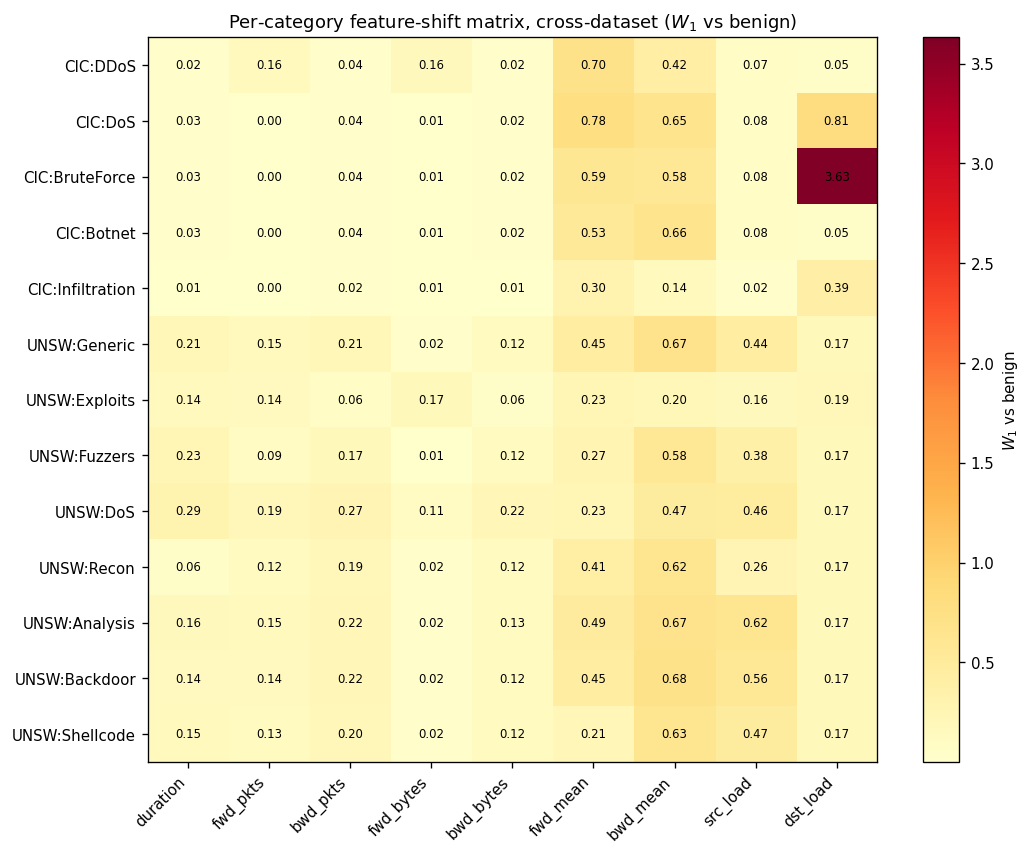
\includegraphics[width=0.92\linewidth]{fig_category_shift_matrix.png}
\caption{Per-category feature-shift matrix, cross-dataset ($W_1$ to benign). Each
row is an attack category from CIC or UNSW; each column is one of the nine SFM
features. The heat pattern is markedly non-uniform both across features within a
category and across the two datasets for nominally comparable categories.}
\label{fig:catshift}
\end{figure}

Two observations confirm the qualitative argument. (i) The dominant shifting
feature is \emph{category-specific}: CIC BruteForce is overwhelmingly driven by
the destination-load (packet-rate) feature ($W_1\!=\!3.63$, far above any other
cell), whereas CIC DDoS is driven by the forward packet-length mean and Botnet by
the backward mean --- so no single feature realignment can serve all categories.
(ii) Nominally comparable categories shift \emph{differently across networks}:
CIC DoS and UNSW DoS have almost identical mean shift ($0.270$ vs $0.269$) yet
concentrate in different features (destination-load for CIC vs.\ flow duration and
packet counts for UNSW), so a calibration tuned on one network's DoS need not
transfer to another's. This empirically substantiates why class-aware few-shot
budgeting --- rather than a single global calibration --- is required for a
rigorous multi-class cross-network deployment, which we develop in future work.

% ============================================================
\section{Conclusion and Future Work}
\label{sec:conclusion}

We presented a systematic cross-network study on the CSE-CIC-IDS2018 and UNSW-NB15
pair. A validated Semantic Feature Mapping enables cross-dataset training; the
combined evidence indicates that the generalization gap is primarily contributed by
a directly measured distribution shift (rather than by a lack of discriminative
information in the shared features), with class-conditional and label-taxonomy
differences as additional factors, and can be closed with low-cost calibration
($1\%$ target labels) or supervised cross-dataset mixup using target train labels,
confirmed on real AWS traffic via few-shot calibration (with the magnitude of the
benefit depending on the evaluation protocol; see Section~\ref{sec:rt-robust}). A
recommended operational configuration is a UNSW-source model plus $\sim$$10\%$
target-domain labels, which nearly matches a model trained fully on the target.

\paragraph{Real-traffic (AWS) validation, in summary.} The cloud experiment
delivers three consistent conclusions. First, under benign-only traffic the
detector is \emph{quiet and stable}: the False Alarm Rate stays below $0.5\%$ and
does not drift with observation length ($0.00\%$ at 3~min $\rightarrow$ $0.38\%$ at
1~h $\rightarrow$ $0.42\%$ over $22{,}644$ benign flows at 6~h), which also rules
out any unit/scaling defect (such bugs spike the FAR toward $100\%$). Second,
\emph{benchmark excellence does not transfer zero-shot}: a model excelling on public
datasets fails to detect real AWS attacks (MCC $\approx 0$; $-0.22$ for the CIC
source), and a three-domain analysis attributes this to genuine distribution shift
(domain-classifier accuracy $\approx 0.99$ among CIC/UNSW/AWS), concentrated in the
rate features (\texttt{src\_load}/\texttt{dst\_load}) and the backward packet size
(\texttt{bwd\_mean}) --- not to a feature or unit error. Third, the shift is
\emph{cheaply repairable}: only $1\%$ AWS labels ($\sim$$107$ flows) lift MCC from
$\approx 0$ to $0.49$, and $10$--$20\%$ reaches $\sim 0.59$, on par with a model
trained entirely on AWS ($0.598$). In short, SFM plus few-shot calibration works on
real cloud traffic, and the recipe can be repeated at each new environment at
minimal labeling cost; we report MCC as the primary metric because AWS-test is
$\approx 99\%$ attack, where F1 would be misleadingly high.

\paragraph{Adversarial robustness and evasion (future direction).} This paper
deliberately \emph{scopes out} adversarial/evasion robustness. In our preliminary
experiments, adversarial training improved in-domain evasion robustness but did
\emph{not} close the cross-network gap --- confirming that adversarial-robustness
and cross-network robustness demand different solutions. A thorough robustness
evaluation --- functional-preserving evasion and adaptive white-box --- is set as
future work in a separate study, on top of the SFM and domain-calibration
foundation validated here.

\paragraph{Automating few-shot labeling in production.} Our AWS labels were derived
from a controlled attack timeline, which is unavailable in a passive real-world
deployment where attack times are unknown. To make the few-shot recipe practical
in production, we propose two complementary label-acquisition paths as future work.
(i) \emph{Active learning}: instead of labeling arbitrary flows, the system selects
only the most \emph{informative} flows --- those nearest the decision boundary or
with highest predictive uncertainty --- and requests labels for a small budget
(tens of flows per drift episode), keeping human effort minimal. (ii)
\emph{SIEM/SOC integration}: labels can be sourced automatically from existing
security infrastructure --- correlation rules and alerts in a SIEM, verdicts from
companion signature-based IDS (e.g., Suricata/Snort), or analyst triage
dispositions in the SOC --- providing weak but low-cost ground truth to drive
few-shot recalibration. A guardrail step (validating any candidate update against a
trusted holdout of known attacks before promotion) would mitigate the risk of
learning attacks as normal.

\paragraph{Other directions.} Having extended the study to multi-class attack
classification in-domain (Section~\ref{sec:multiclass}), the remaining directions
are: (i) \emph{multi-class detection on real cloud traffic}, using per-category
labels reconstructed from the attack timeline, and class-aware few-shot budgeting
for the rare categories that our per-category analysis shows to be hardest;
(ii) \emph{online/streaming continuous adaptation} with concept-drift detection so
the model recalibrates itself over extended multi-day deployment without full
retraining --- the natural successor to the one-shot few-shot recipe here;
(iii) robust ensembles under edge compute budgets and stronger domain adaptation to
address the direction asymmetry. Adversarial robustness is pursued separately (see
above).

% ============================================================
\section*{CRediT authorship contribution statement}
\textbf{Hero Yudo Martono}: Conceptualization, Methodology, Software,
Investigation, Data curation, Writing --- original draft. \textbf{Iwan Syarif}:
Supervision, Methodology, Writing --- review \& editing. \textbf{Ferry Astika
Saputra}: Supervision, Validation, Writing --- review \& editing.

\section*{Declaration of competing interest}
The authors declare that they have no known competing financial interests or
personal relationships that could have appeared to influence the work reported in
this paper.

\section*{Declaration of generative AI and AI-assisted technologies}
During the preparation of this work the authors used AI-assisted tools to help
with language editing and LaTeX formatting. After using these tools, the authors
reviewed and edited the content as needed and take full responsibility for the
content of the published article. No generative AI tools were used to create or
alter primary research data or experimental result figures; all data
visualizations are derived directly from the underlying experimental data via
reproducible analytical methods.

\section*{Data availability}
This study uses two public benchmark datasets: CSE-CIC-IDS2018 (Canadian Institute
for Cybersecurity) and UNSW-NB15 (UNSW Canberra), both available from their
respective official providers. The real-traffic AWS validation flows were
generated by the authors in a controlled environment. The code, configuration,
notebooks, and compact result artifacts (feature-mapping tables, extracted flow
features, and analysis notebooks) that support the findings are publicly available
at \url{https://github.com/heroyudo-gmail/kiro-ssh} (subfolder \texttt{unswnb-15/}).

% ============================================================
\begin{thebibliography}{99}

\bibitem[Cremer et al.(2022)]{cremer}
F.~Cremer, B.~Sheehan, M.~Fortmann, A.~N.~Kia, M.~Mullins, F.~Murphy, S.~Materne,
Cyber risk and cybersecurity: A systematic review of data availability,
\textit{Geneva Papers Risk Insurance --- Issues Pract.} 47 (3) (2022) 698--736.

\bibitem[Torres et al.(2019)]{torres}
J.~M.~Torres, C.~I.~Comesa\~na, P.~J.~Garc\'ia-Nieto, Machine learning techniques
applied to cybersecurity, \textit{Int.\ J.\ Mach.\ Learn.\ Cybern.} 10 (10) (2019)
2823--2836.

\bibitem[Sarker et al.(2020)]{sarker}
I.~H.~Sarker, A.~S.~M.~Kayes, S.~Badsha, H.~Alqahtani, P.~Watters, A.~Ng,
Cybersecurity data science: An overview from machine learning perspective,
\textit{J.\ Big Data} 7 (1) (2020) 1--29.

\bibitem[Khraisat et al.(2019)]{khraisat}
A.~Khraisat, I.~Gondal, P.~Vamplew, J.~Kamruzzaman, Survey of intrusion detection
systems: Techniques, datasets and challenges, \textit{Cybersecurity} 2 (1) (2019)
1--22.

\bibitem[Buczak and Guven(2016)]{buczak}
A.~L.~Buczak, E.~Guven, A survey of data mining and machine learning methods for
cyber security intrusion detection, \textit{IEEE Commun.\ Surveys Tuts.} 18 (2)
(2016) 1153--1176.

\bibitem[Bhuyan et al.(2014)]{bhuyan}
M.~H.~Bhuyan, D.~K.~Bhattacharyya, J.~K.~Kalita, Network anomaly detection:
Methods, systems and tools, \textit{IEEE Commun.\ Surveys Tuts.} 16 (1) (2014)
303--336.

\bibitem[Tavallaee et al.(2009)]{kdd}
M.~Tavallaee, E.~Bagheri, W.~Lu, A.~A.~Ghorbani, A detailed analysis of the KDD
Cup 99 data set, in: Proc.\ IEEE CISDA, 2009, pp.~1--6.

\bibitem[Moustafa and Slay(2015)]{unsw}
N.~Moustafa, J.~Slay, UNSW-NB15: A comprehensive data set for network intrusion
detection systems, in: Proc.\ MilCIS, 2015, pp.~1--6.

\bibitem[Moustafa and Slay(2016)]{unsweval}
N.~Moustafa, J.~Slay, The evaluation of network anomaly detection systems:
Statistical analysis of the UNSW-NB15 data set and the comparison with the KDD99
data set, \textit{Inf.\ Secur.\ J.} 25 (1--3) (2016) 18--31.

\bibitem[Sharafaldin et al.(2018)]{cicids}
I.~Sharafaldin, A.~H.~Lashkari, A.~A.~Ghorbani, Toward generating a new intrusion
detection dataset and intrusion traffic characterization, in: Proc.\ ICISSP, 2018,
pp.~108--116.

\bibitem[Sharafaldin et al.(2019)]{cicddos}
I.~Sharafaldin, A.~H.~Lashkari, S.~Hakak, A.~A.~Ghorbani, Developing realistic
distributed denial of service (DDoS) attack dataset and taxonomy, in: Proc.\ ICCST,
2019, pp.~1--8.

\bibitem[Koroniotis et al.(2019)]{botiot}
N.~Koroniotis, N.~Moustafa, E.~Sitnikova, B.~Turnbull, Towards the development of
realistic botnet dataset for IoT networks, \textit{IEEE Access} 7 (2019)
94529--94541.

\bibitem[Alsaedi et al.(2020)]{toniot}
A.~Alsaedi, N.~Moustafa, Z.~Tari, A.~N.~Mahmood, A.~Anwar, TON\_IoT telemetry
dataset, \textit{IEEE Access} 8 (2020) 165130--165150.

\bibitem[Neto et al.(2023)]{ciciot}
E.~C.~P.~Neto, S.~Dadkhah, R.~Ferreira, A.~Zohourian, R.~Lu, A.~A.~Ghorbani,
CICIoT2023: A real-time dataset and benchmark for large-scale attacks in IoT
environment, \textit{Sensors} 23 (13) (2023) art.~5941.

\bibitem[Ring et al.(2019)]{ring}
M.~Ring, S.~Wunderlich, D.~Scheuring, D.~Landes, A.~Hotho, A survey of
network-based intrusion detection data sets, \textit{Comput.\ Secur.} 86 (2019)
147--167.

\bibitem[Engelen et al.(2021)]{engelen}
G.~Engelen, V.~Rimmer, W.~Joosen, Troubleshooting an intrusion detection dataset:
The CICIDS2017 case study, in: Proc.\ IEEE SPW, 2021, pp.~7--12.

\bibitem[Rosay et al.(2022)]{rosay}
A.~Rosay, E.~Cheval, F.~Carlier, P.~Leroux, Network intrusion detection: A
comprehensive analysis of CIC-IDS2017, in: Proc.\ ICISSP, 2022, pp.~25--36.

\bibitem[Lanvin et al.(2022)]{lanvin}
M.~Lanvin, P.-F.~Gimenez, Y.~Han, F.~Majorczyk, L.~M\'e, \'E.~Totel, Errors in the
CICIDS2017 dataset and the significant differences in detection performances it
makes, in: Proc.\ CRiSIS, 2022, pp.~18--33.

\bibitem[Liu et al.(2022)]{liu}
L.~Liu, G.~Engelen, T.~Lynar, D.~Essam, W.~Joosen, Error prevalence in NIDS
datasets: A case study on CIC-IDS-2017 and CSE-CIC-IDS-2018, in: Proc.\ IEEE CNS,
2022, pp.~254--262.

\bibitem[Catillo et al.(2023)]{catillo}
M.~Catillo, A.~Pecchia, U.~Villano, Machine learning on public intrusion datasets:
Academic hype or concrete advances in NIDS?, in: Proc.\ IEEE/IFIP DSN-S, 2023,
pp.~132--136.

\bibitem[Layeghy et al.(2024)]{layeghy}
S.~Layeghy, M.~Gallagher, M.~Portmann, Benchmarking the benchmark --- Comparing
synthetic and real-world network IDS datasets, \textit{J.\ Inf.\ Secur.\ Appl.} 80
(2024) art.~103689.

\bibitem[Sarhan et al.(2022a)]{sarhan}
M.~Sarhan, S.~Layeghy, M.~Portmann, Towards a standard feature set for network
intrusion detection system datasets, \textit{Mobile Netw.\ Appl.} 27 (1) (2022)
357--370.

\bibitem[Sarhan et al.(2022b)]{sarhannf}
M.~Sarhan, S.~Layeghy, N.~Moustafa, M.~Portmann, NetFlow datasets for machine
learning-based network intrusion detection systems, in: Big Data Technologies and
Applications, Springer, 2022.

\bibitem[Cantone et al.(2024)]{cantone}
M.~Cantone, C.~Marrocco, A.~Bria, Machine learning in network intrusion detection:
A cross-dataset generalization study, \textit{IEEE Access} 12 (2024)
144491--144509.

\bibitem[D'Hooge et al.(2020)]{dhooge}
L.~D'Hooge, T.~Wauters, B.~Volckaert, F.~De~Turck, Inter-dataset generalization
strength of supervised machine learning methods for intrusion detection,
\textit{J.\ Inf.\ Secur.\ Appl.} 54 (2020) art.~102564.

\bibitem[Verkerken et al.(2022)]{verkerken}
M.~Verkerken, L.~D'Hooge, T.~Wauters, B.~Volckaert, F.~De~Turck, Towards model
generalization for intrusion detection: Unsupervised machine learning techniques,
\textit{J.\ Netw.\ Syst.\ Manage.} 30 (1) (2022) 1--25.

\bibitem[Popoola et al.(2021)]{popoola}
S.~I.~Popoola, G.~Gui, B.~Adebisi, M.~Hammoudeh, H.~Gacanin, Federated deep
learning for collaborative intrusion detection in heterogeneous networks, in:
Proc.\ IEEE VTC-Fall, 2021, pp.~1--6.

\bibitem[de Carvalho Bertoli et al.(2023)]{bertoli}
G.~de~Carvalho~Bertoli, L.~A.~Pereira~Jr., O.~Saotome, A.~L.~dos~Santos,
Generalizing intrusion detection for heterogeneous networks: A stacked-unsupervised
federated learning approach, \textit{Comput.\ Secur.} 127 (2023) art.~103106.

\bibitem[Agrawal et al.(2022)]{agrawal}
S.~Agrawal, S.~Sarkar, O.~Aouedi, G.~Yenduri, K.~Piamrat, M.~Alazab,
S.~Bhattacharya, P.~K.~R.~Maddikunta, T.~R.~Gadekallu, Federated learning for
intrusion detection system: Concepts, challenges and future directions,
\textit{Comput.\ Commun.} 195 (2022) 346--361.

\bibitem[Wang et al.(2024)]{nidsfgpa}
J.~Wang, K.~Yang, M.~Li, NIDS-FGPA: A federated learning network intrusion
detection algorithm based on secure aggregation of gradient similarity models,
\textit{PLoS ONE} 19 (10) (2024) art.~e0308639.

\bibitem[Chen and Guestrin(2016)]{xgboost}
T.~Chen, C.~Guestrin, XGBoost: A scalable tree boosting system, in: Proc.\ ACM
SIGKDD, 2016, pp.~785--794.

\bibitem[Husain et al.(2019)]{husain}
A.~Husain, A.~Salem, C.~Jim, G.~Dimitoglou, Development of an efficient network
intrusion detection model using XGBoost on the UNSW-NB15 dataset, in: Proc.\ IEEE
ISSPIT, 2019, pp.~1--7.

\bibitem[Zhou et al.(2020)]{zhou}
Y.~Zhou, G.~Cheng, S.~Jiang, M.~Dai, Building an efficient intrusion detection
system based on feature selection and ensemble classifier, \textit{Comput.\ Netw.}
174 (2020) art.~107247.

\bibitem[Shone et al.(2018)]{shone}
N.~Shone, T.~N.~Ngoc, V.~D.~Phai, Q.~Shi, A deep learning approach to network
intrusion detection, \textit{IEEE Trans.\ Emerg.\ Topics Comput.\ Intell.} 2 (1)
(2018) 41--50.

\bibitem[Liu and Lang(2019)]{liulang}
H.~Liu, B.~Lang, Machine learning and deep learning methods for intrusion
detection systems: A survey, \textit{Appl.\ Sci.} 9 (20) (2019) art.~4396.

\bibitem[Mahdavifar and Ghorbani(2019)]{mahdavifar}
S.~Mahdavifar, A.~A.~Ghorbani, Application of deep learning to cybersecurity: A
survey, \textit{Neurocomputing} 347 (2019) 149--176.

\bibitem[Wu et al.(2022)]{wu}
Z.~Wu, H.~Zhang, P.~Wang, Z.~Sun, RTIDS: A robust transformer-based approach for
intrusion detection system, \textit{IEEE Access} 10 (2022) 64375--64387.

\bibitem[Duan et al.(2023)]{duan}
G.~Duan, H.~Lv, H.~Wang, G.~Feng, Application of a dynamic line graph neural
network for intrusion detection with semisupervised learning, \textit{IEEE
Transactions on Information Forensics and Security} 18 (2023) 699--714.


\bibitem[Sun et al.(2016)]{coral}
B.~Sun, J.~Feng, K.~Saenko, Return of frustratingly easy domain adaptation, in:
Proc.\ AAAI, 2016, pp.~2058--2065.

\bibitem[Ben-David et al.(2010)]{bendavid}
S.~Ben-David, J.~Blitzer, K.~Crammer, A.~Kulesza, F.~Pereira, J.~W.~Vaughan, A
theory of learning from different domains, \textit{Mach.\ Learn.} 79 (1--2) (2010)
151--175.

\bibitem[Xu et al.(2025)]{fewshot}
C.~Xu, Y.~Zhan, G.~Chen, Z.~Wang, S.~Liu, W.~Hu, Elevated few-shot network
intrusion detection via self-attention mechanisms and iterative refinement,
\textit{PLoS ONE} 20 (1) (2025) art.~e0317713.

\bibitem[Villani(2009)]{wasserstein}
C.~Villani, \textit{Optimal Transport: Old and New}, Springer, 2009.

\bibitem[Pedregosa et al.(2011)]{sklearn}
F.~Pedregosa et al., Scikit-learn: Machine learning in Python, \textit{J.\ Mach.\
Learn.\ Res.} 12 (2011) 2825--2830.

\bibitem[Kohavi(1995)]{kohavi}
R.~Kohavi, A study of cross-validation and bootstrap for accuracy estimation and
model selection, in: Proc.\ IJCAI, 1995, pp.~1137--1143.

\bibitem[Matthews(1975)]{matthews}
B.~W.~Matthews, Comparison of the predicted and observed secondary structure of T4
phage lysozyme, \textit{Biochim.\ Biophys.\ Acta} 405 (2) (1975) 442--451.

\bibitem[Chicco and Jurman(2020)]{chicco}
D.~Chicco, G.~Jurman, The advantages of the Matthews correlation coefficient (MCC)
over F1 score and accuracy in binary classification evaluation, \textit{BMC
Genomics} 21 (1) (2020) 6.

\end{thebibliography}

\end{document}
